\documentclass[conference]{IEEEtran}
%\IEEEoverridecommandlockouts
% The preceding line is only needed to identify funding in the first footnote. If that is unneeded, please comment it out.
\usepackage{cite}
\usepackage{amsmath,amssymb,amsfonts}
\usepackage{algorithmic}
\usepackage{graphicx}
\usepackage{textcomp}
\usepackage{xcolor}

\usepackage{url}
\usepackage{hyperref}

\def\BibTeX{{\rm B\kern-.05em{\sc i\kern-.025em b}\kern-.08em
    T\kern-.1667em\lower.7ex\hbox{E}\kern-.125emX}}
\begin{document}

\title{ATSC - A novel approach to monitoring time series compression\\}

\author{\IEEEauthorblockN{1\textsuperscript{st} Carlos Rolo}
\IEEEauthorblockA{\textit{Instaclustr (of Aff.)} \\
\textit{Netapp (of Aff.)}\\
Lisbon, Portugal \\
carlos.rolo@netapp.com}
\and
\IEEEauthorblockN{2\textsuperscript{nd} Joshua Varghese}
\IEEEauthorblockA{\textit{dept. name of organization (of Aff.)} \\
\textit{Open SI(NetApp)}\\
Canberra, Australia \\
u3227463@uni.canberra.edu.au}
}

\maketitle

\begin{abstract}
    This research paper introduces an innovative approach to time series compression tailored for the complexities of computer systems monitoring. The Advanced Time Series Compression (ATSC) methodology, drawing inspiration from established audio compression techniques, achieves significant compression ratios, potentially resulting in space savings of up to 57.34 times. With a strong emphasis on precise data retrieval and efficient streaming capabilities, ATSC presents a promising solution for effectively managing high-frequency time series data within the realm of computer systems monitoring. The study underscores the critical importance of unique indexing for targeted decompression and showcases promising results from initial testing against traditional methods. Future research directions encompass exploring automated selections, integration with time series databases, and further optimization for enhanced efficiency. ATSC emerges as an innovative and forward-thinking solution that not only addresses current challenges in storage and data transfer but also propels advancements in time series monitoring and data compression within computer systems.
\end{abstract}
\vspace{5pt}
\begin{IEEEkeywords}
Timeseries Compression, Function Approximation, Audio Compression, Data Storage, Streaming, Indexing, Computer Systems Monitoring
\end{IEEEkeywords}

\section{Introduction}
The realm of computer systems monitoring, distinct from general time-series monitoring, is characterized by a unique set of challenges. Typically marked by very low-frequency sampling, ranging from 0.05Hz to 1~2Hz, this process focuses on capturing signals from various processes, such as database operations and the overall health of the operating system [10]. 
 
An intriguing facet of this domain is the absence of periodicity or harmonic components in most signals. In many cases, these signals are treated as isolated samples or short sequences, employing compression techniques like XOR compression and delta-delta encoding. 
However, a paradigm shift emerges by viewing these signals collectively. While the techniques themselves may not be novel, their application in this domain is ground-breaking. By harnessing audio packing and processing methodologies, we not only capitalize on compression benefits but also tap into the extensive streaming functionality embedded in audio formats. 
 
The significance of data compression extends beyond storage concerns to encompass in-transit scenarios, especially with the rise of cloud computing. Sending monitoring data to external systems incurs egress costs, and stored data must be uncompressed and processed before transmission. Leveraging audio packing techniques allows us to seamlessly integrate with the broader ecosystem of software and hardware, ranging from servers to mobile devices, proficient in transporting and encoding/decoding such information on demand. 

\begin{figure}[h]
  \centering
  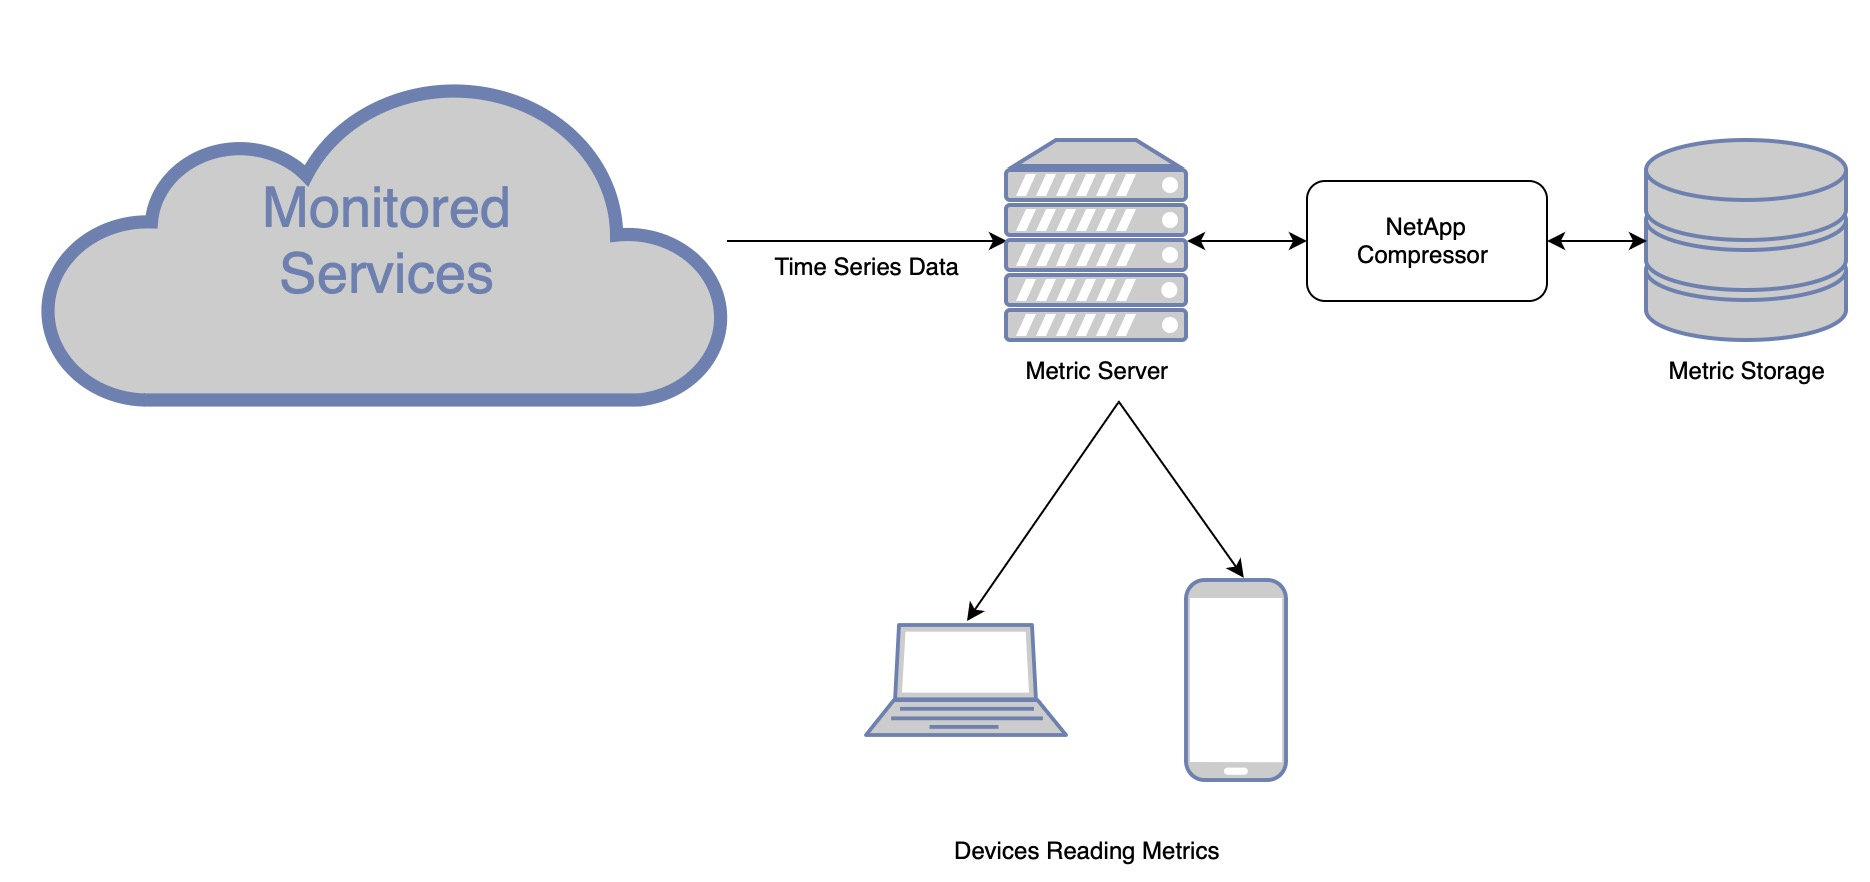
\includegraphics[width=0.5\textwidth]{Fig1.png}
  \caption{Flow of data from monitored services to devices reading metrics.}
  \label{Fig.1}
\end{figure}

Our approach doesn't only yield savings in at-rest scenarios but also in transit and during compute processing. By having the ability to leverage client-side devices [9], we enable efficient processing and transport of monitoring data. Integration in system-on-a-Chip architectures [8] could lead to further performance enhancements. This strategy positions our methodology at the forefront of efficient and resource-conscious computer systems monitoring. ATSC address this issues while keeping Compression and Decompression speed and resource consumption at a similar level as current existing compression algorithms.

\section{Background}

In the dynamic landscape of computer systems monitoring, the impetus for our research stems from critical challenges that impact both the efficiency and cost-effectiveness of current practices. 

\subsection{High Storage Cost}

The exponential growth of data in computer systems monitoring has led to soaring storage costs. Traditional methods often struggle to cope with the sheer volume of information generated by processes, databases, and overall system health monitoring. Our research delves into innovative time-series compression techniques to alleviate the burden of high storage costs, offering a sustainable solution for data retention. 

\subsection{High Egress Cost}
Sending monitoring data to external systems, especially in cloud environments, incurs in egress costs. Our research recognises the financial implications of these expenses and aims to mitigate them through advanced compression methodologies. By optimising data before transmission, we not only reduce egress costs but also enhance the overall efficiency of data transfer. 

\subsection{Balancing Data Reduction and Information Preservation}
To manage overwhelming data volumes, conventional practices often resort to techniques like averaging, sub-sampling or by not collecting enough information via very low sampling. While effective in reducing data points, this approach comes at a cost – a loss of valuable information. Our research seeks to address this trade-off by proposing advanced time-series compression methods that achieve data reduction without sacrificing critical insights and information. 

\subsection{Computational Challenges in Traditional Monitoring Techniques}
Traditional approaches, such as point-walking algorithms, demand substantial computational resources to process the vast amounts of monitoring data. Recognising the strain on computing capabilities, our research introduces a more resource-efficient paradigm. By exploring novel compression techniques inspired by audio processing, we aim to streamline the computational demands of data analysis in computer systems monitoring. 

  
\begin{figure}[h]
  \centering
  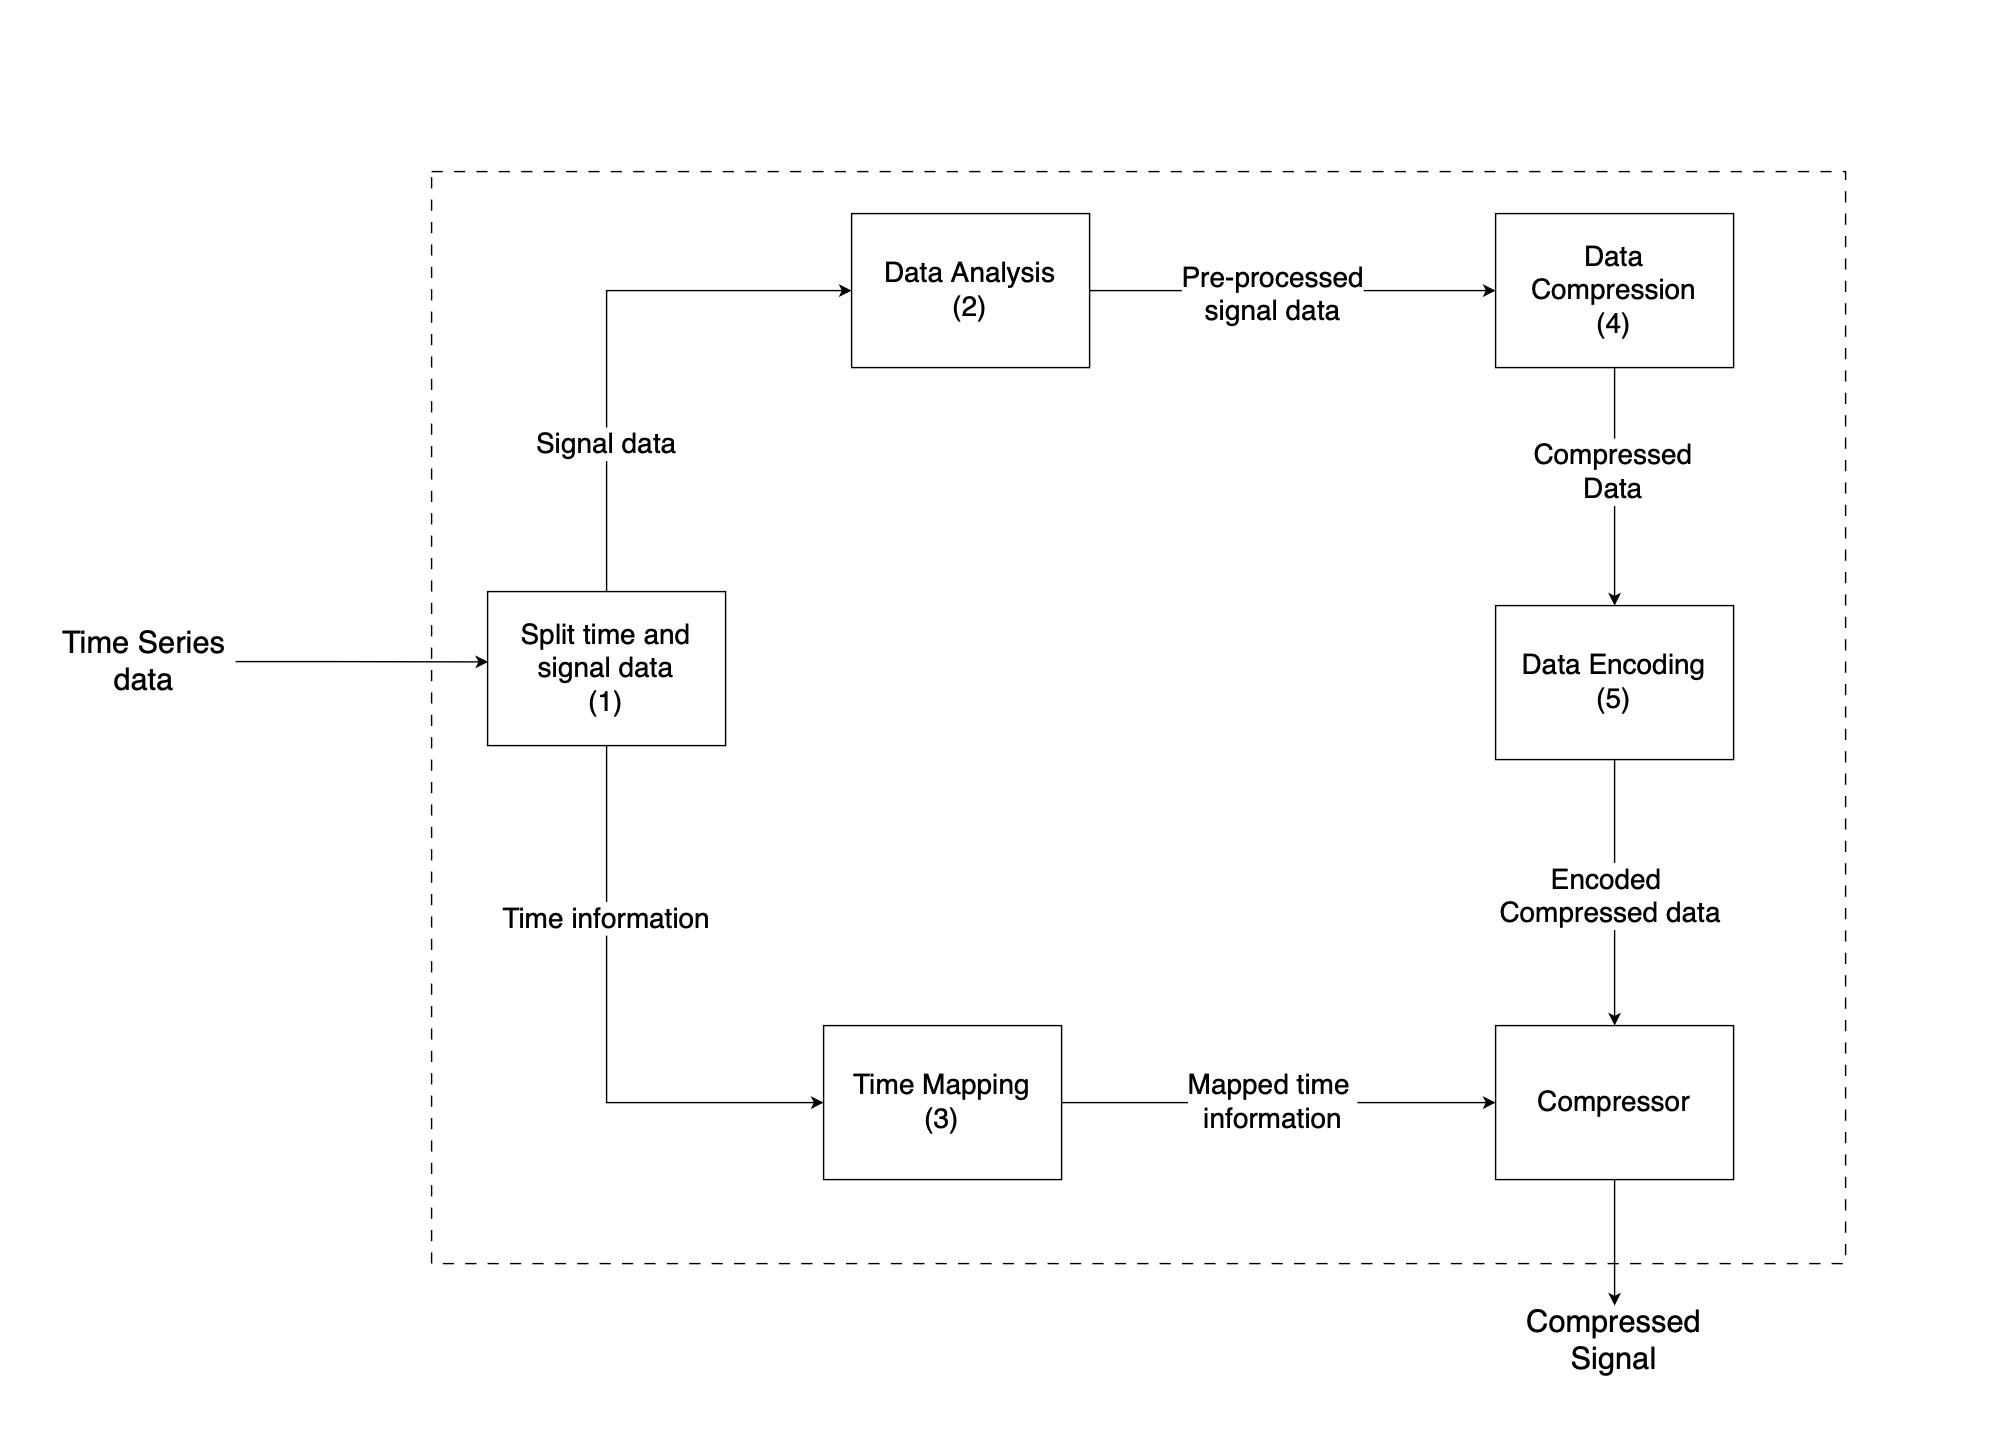
\includegraphics[width=0.5\textwidth]{Fig2.png}
  \caption{Architecture of computer system.}
  \label{Fig.2}
\end{figure}

Our comprehensive approach not only tackles the immediate challenges of high storage and egress costs but also addresses the inherent trade-offs in data reduction techniques. The overarching goal is to improve the landscape of computer systems monitoring by introducing a cost-effective and information-rich paradigm through advanced time-series compression. 



\section{Architecture}

\subsection{ATSC Write Paths}

\subsubsection{Pre-processing the Signal for Initial Reduction}
Ahead of compression, the signal undergoes a statistical pre-processing, calculating means, variance, etc. This initial step aims to eliminate redundant information and prepare the signal for more advanced compression methodologies.

\vspace{10pt}
\subsubsection{Packing the Signal in a Non-compressed Format (WAVBRO)}
The uncompressed signal may then be packed into a non-compressed format. For this we created a new format heavily inspired by WAV. The signal can also be stored in the WAV format, but for this frequency might need to be converted, since WAV doesn't support <1 HZ frequencies. Additionally, the signal might be strategically split into integer and float types formatted to sizes compatible with audio sampling. Also, the signal might be split into different channels to reduce size. 

\vspace{10pt}
\subsubsection{Identifying and Exploiting Local Opportunities within the signal}
ATSC leverages its distinctive approach by identifying local opportunities that are more suitable for a mathematical approximation. By slicing the signal in a targeted way, this sets the stage for enhanced compression in the subsequent stages. One way of doing such slicing is via Wavelets transforms, so that high and low frequencies components are identified and the signal divided in different parts accordingly to its behaviour.
In case a clear opportunity for slicing the samples in optimal blocks are not identified, blocks are created with an optimal size for FFT processing (in the form of $slice = 2^n * 3^m$).

\begin{figure}[ht]
  \centering
  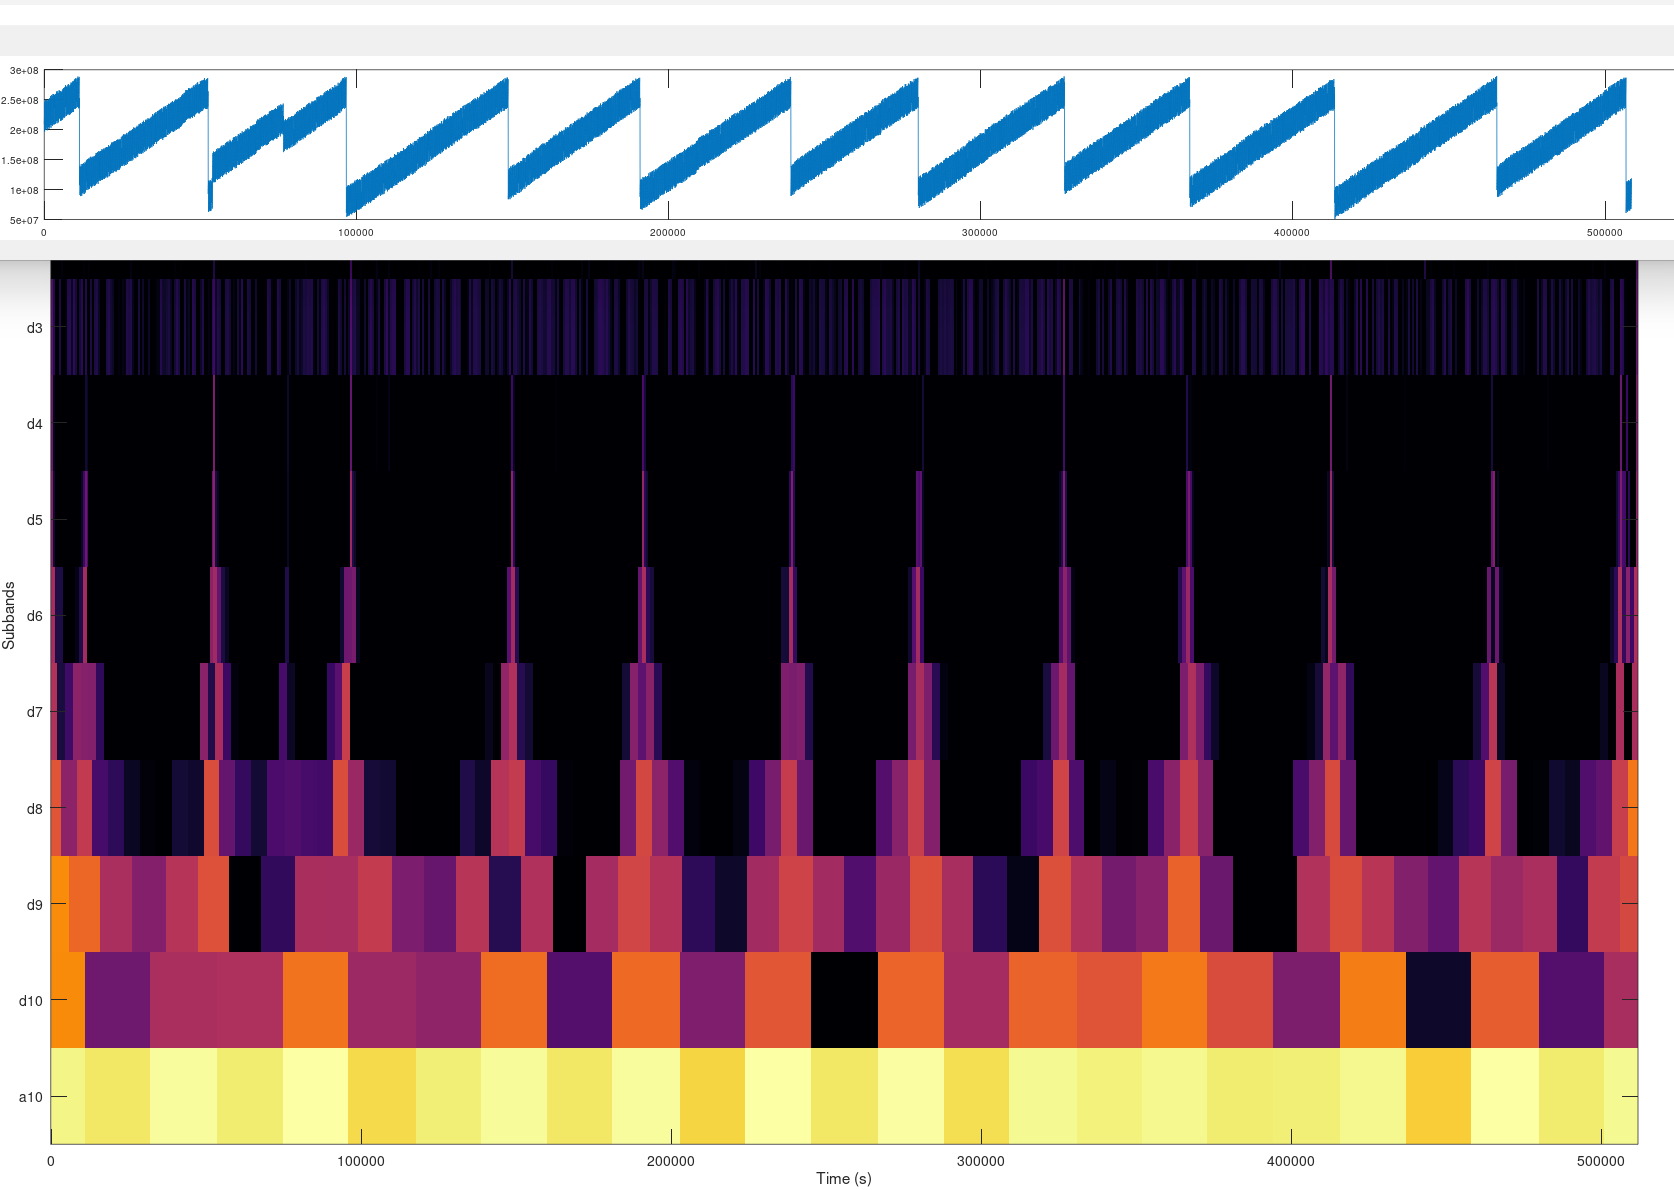
\includegraphics[width=0.5\textwidth]{wavelet_heap.png}
  \caption{Example of wavelet detection of high frequency sections to slice the signal. Signal on top and Wavelet Analysis on bottom.}
  \label{Fig.3}
\end{figure}
\vspace{5pt}

\vspace{10pt}
\subsubsection{Generate an Index for Precision Access}
To facilitate precise access to samples without the need for full file seeking or decompression of the full file, ATSC generates a comprehensive index. This index ensures efficient retrieval of relevant portions of the signal, a critical aspect in the subsequent compression and decompression processes.

\vspace{10pt}
\subsubsection{Blocking and Modelling}
The signal samples are divided into blocks, and for each block, ATSC applies modelling techniques tailored to the specific characteristics of the signal. This may involve techniques such as Linear Predictive Coding (LPC), Polynomial Prediction, Fast Fourier Transforms (FFT), or other methodologies that best suit the signal's behaviour. This modeling converts the original samples into an approximated formula. In some cases it is possible to match the original signal precisely. This leads to a high number of data points being converted into a mathematical formula and its components.

\vspace{10pt}
\subsubsection{Error correction and final optimizations}
In cases where the resulting formulas are approximated, error correction can be applied. A error percentage can be provided so that the amount of error correction is applied until the approximation + error correction falls within the provided error margin. After the error corrections are applied (either via keeping samples with the highest error, Huffman-codding differences, etc) further optimization is done by reducing the information to the minimal computational size needed for each sample. Samples are normally provided in 64bits size, this step can reduce the sample size to 8bit if the samples fit.

\vspace{10pt}
\subsubsection{Generate the Final Compressed File}
Building upon the insights gained from steps 1 to 7, ATSC culminates the write path by generating the final compressed file. This file encapsulates the intricacies of the original signal in a highly compressed and efficient format, ready for storage or transmission.


\subsection{ATSC Read Paths}

ATSC distinguishes itself by eschewing the storage of timestamp information directly within the file, opting instead for a distinctive indexing approach that enables efficient streaming and targeted decompression of pertinent data segments.
Within the Read Path of ATSC, the samples are located via an indexing table, and then uncompressed, or the full content if requested. 
Since speed is important in retrieval of metrics, the read stage, after the location of the samples, applies the mathematical formula defined for the sample segment plus any error correction, and the returns the samples. 

\vspace{10pt}
\subsubsection{Precise Streaming through Specialized Indexing}\label{SCMA}
The core innovation in the Read Path lies in the application of a specialized indexing mechanism. Unlike traditional methods, ATSC's indexing facilitates pinpointing the relevant portion of the file without the necessity of timestamp inclusion in the file itself. This precision in indexing empowers ATSC to streamline the streaming process, focusing exclusively on the required data, thereby optimizing resource utilization. 

\vspace{10pt}
\subsubsection{Unveiling of the Read Path}\label{SCMC}
\begin{itemize}

\item{\textbf{\textit{Identifying the Samples to be Retrieved:}}} The Read Path initiation begins with the user specifying time interval of metric of interest. If no interval is provided, all samples are returned.

\vspace{5pt}
\item{\textbf{\textit{Precision in Data Retrieval Using the Index:}}} The index plays a crucial role in ATSC's approach. It aids in precisely identifying the segment of the file essential for the query. This ensures focused and efficient data retrieval.

\vspace{5pt}
\item{\textbf{\textit{Sample decompression:}}} Once the relevant data segment is identified, ATSC initiates the decompression of the data.
For the located data samples, the correspondent formula translation is applied and any error correction.

\vspace{5pt}
\item{\textbf{\textit{Timestamp Integration Post-Decompression:}}} Following decompression, the samples, now in their extracted form, receive timestamp information from the index. This final step ensures temporal accuracy and relevance of the retrieved data.

\vspace{5pt}
\item{\textbf{\textit{Streaming/Writting data out:}}} Under a streaming process, samples are sent while being decompressed. ATSC also supports full file decompression where all the data is decompressed and then send out, or written out to a WAVBRO file.
\end{itemize}

\section{Compression Methods}

Mostly of the work is done in this step. After a statistical analysis the signal, the compressor stage decides which approach is best for a given block of samples.
Things like first and second derivative analysis also allows a more precise selection of the compression form. 
For example, a signal which is mostly stable (small variation) will be approximated by a Spline, a signal with a lot of variation will be better approximated by an Fast Fourier Transform or a Linear Predictive Coding.

\vspace{10pt}
\subsubsection{Fast Fourier Transforms (FFT)}

Compression with FFT is done via a conversion of the signal to the frequency domain. Once in the frequency domain, we store a subset of frequencies.
The number of frequencies selected depends on the error margin we want to store the signal with. Since the signals are always real, the worst case scenario (lossless compression) half the frequencies need to be stored.
But since every frequency is represented by a pair of (Real, Imaginary) values, the lossless compression is next to none. 
The frequency pairs are always represented by two floats, either 32 or 64 bits depending on the precision required.
In a lossy scenario, and depending on the signal, 10x reduction in size is easily achievable within a 1\% to 3\% error margin.
To decompress, the Inverse FFT is applied on the available frequencies, zeroing out the missing frequencies.

\begin{figure}[ht]
  \centering
  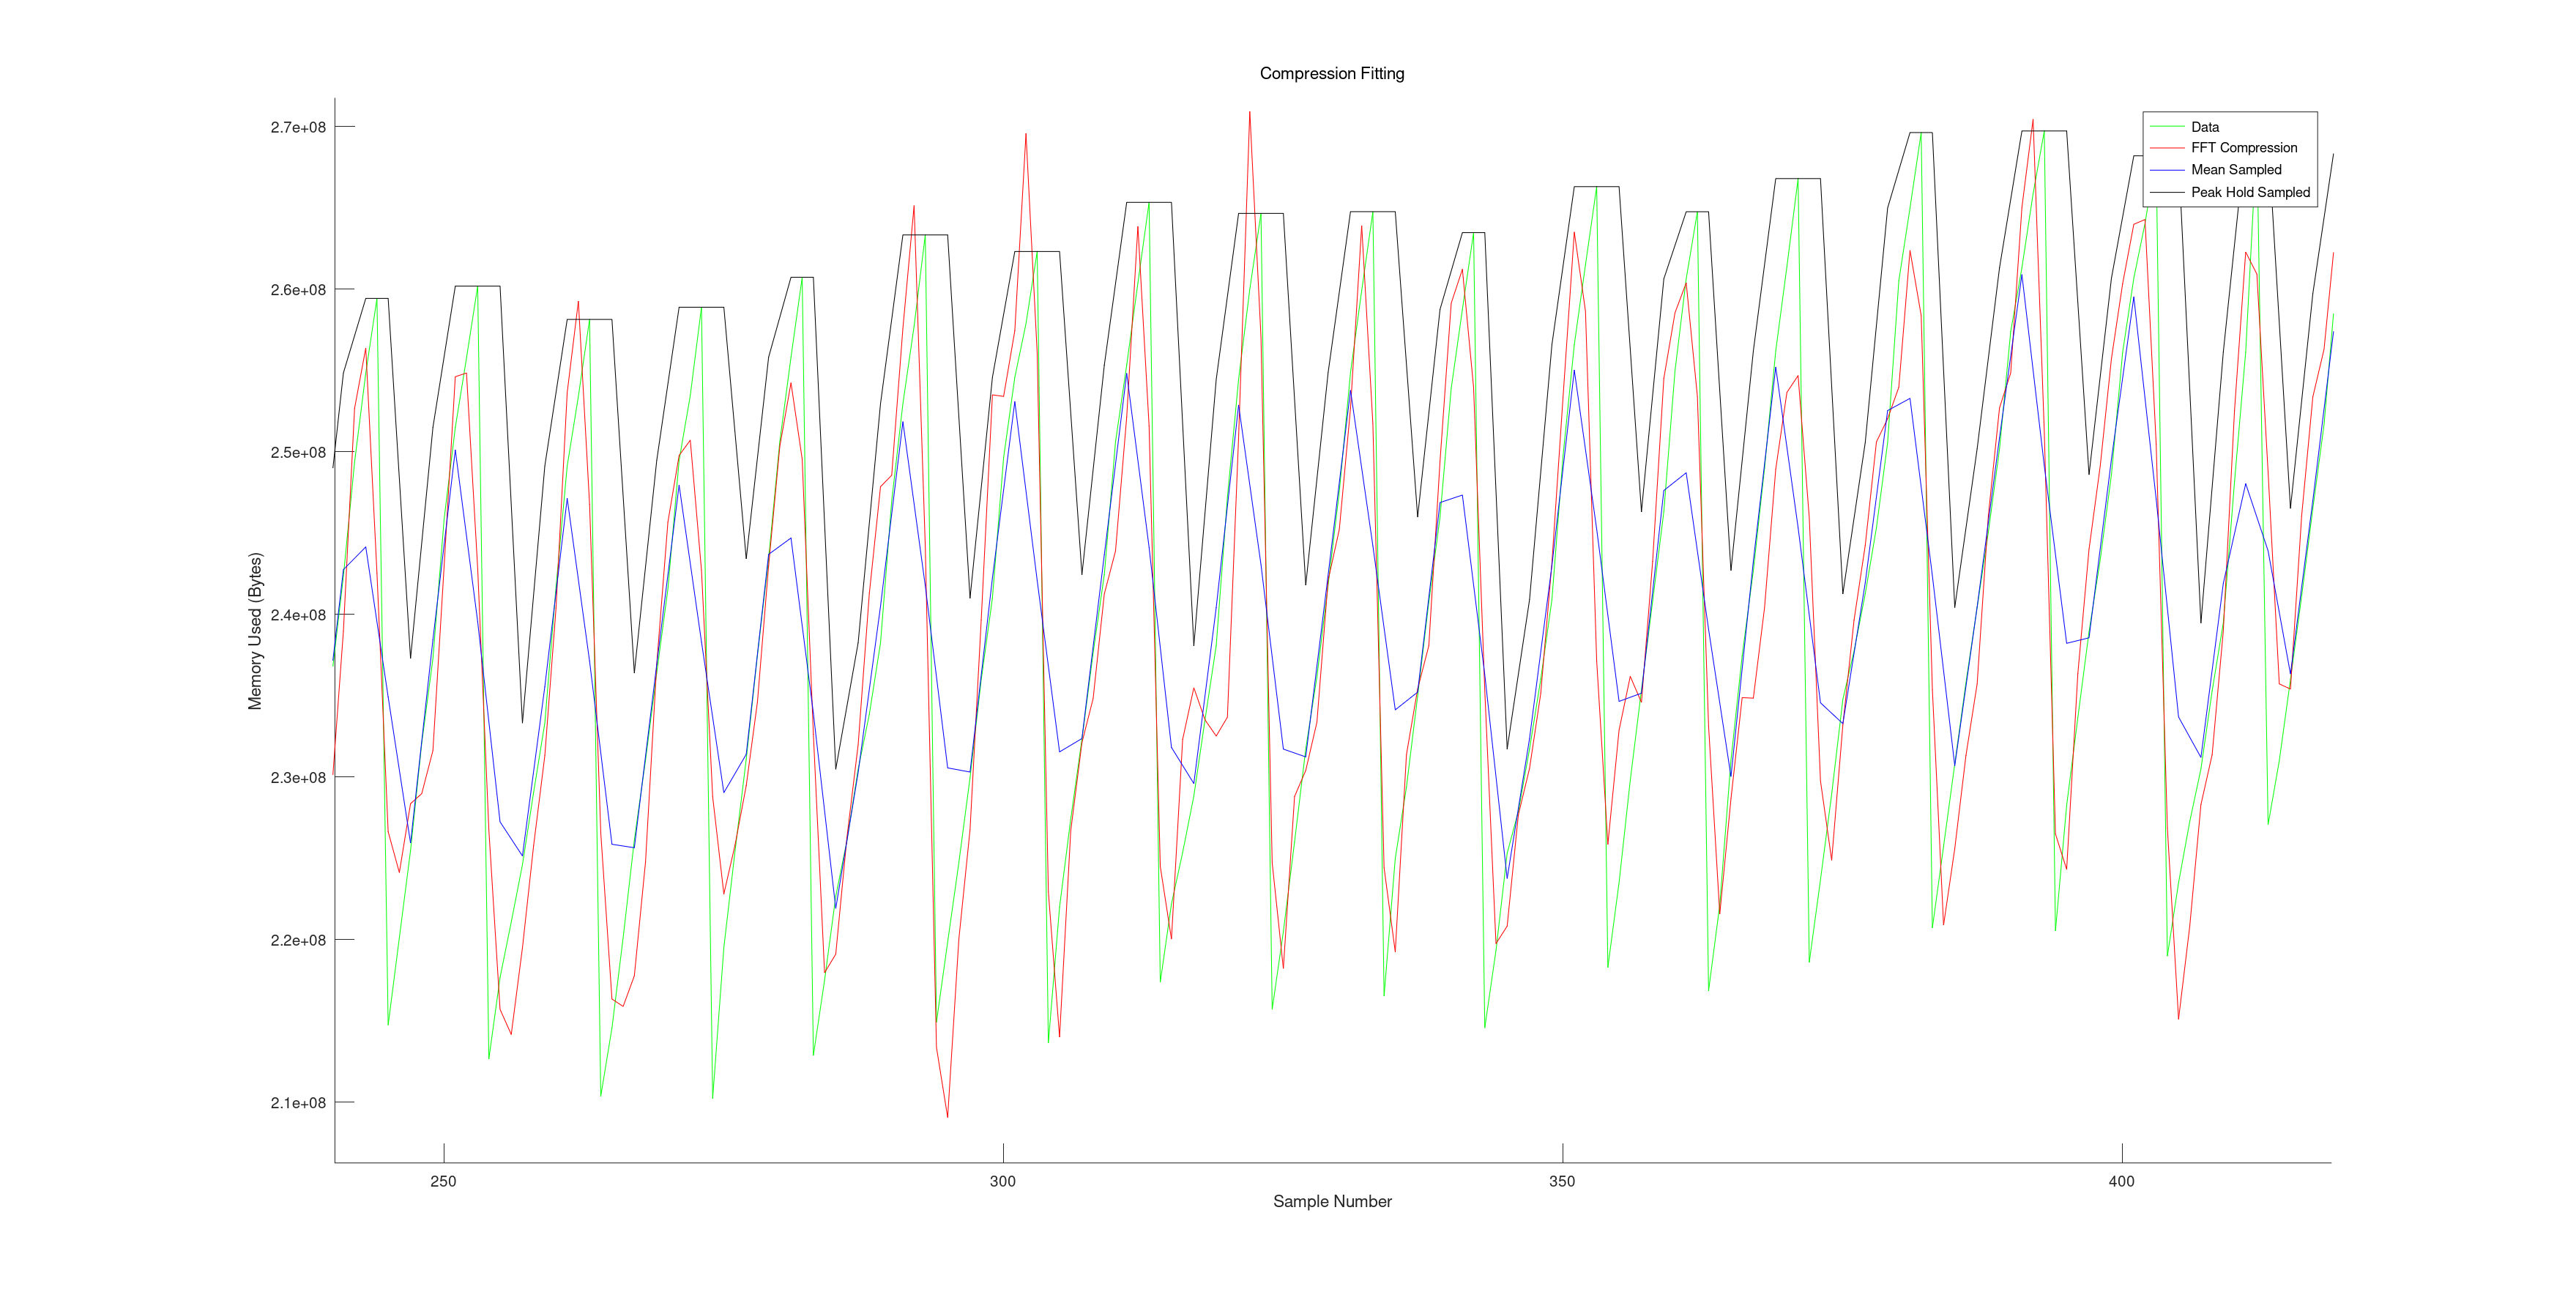
\includegraphics[width=0.5\textwidth]{FFT_Comparison.png}
  \caption{Signal Fitting of the original data vs FFT Compression (8x compression) vs Average Sampled (2x) and Peak Hold (2x).}
  \label{Fig.3}
\end{figure}
\vspace{5pt}

\subsubsection{Spline Interpolation}

Another compression method is via a Spline Interpolation. Currently using either linear for simple signals (near-linear signals like Disk usage) or Catmull-Rom interpolation for everything else.
The method is similar to the FFT, where several points are stored and the corresponding outputs calculated via Spline Interpolation.
Once a Spline is generated within the margin of error provided, the points that generated that spline are stored.
An advantage of Spline Interpolation vs FFT is that the FFT always need to store the data as a pair of floats. 
While the Spline Interpolation the points are the same as the data points, so a integer signal would be stored as integer with the same bit depth as the original signal.
This could be something as small as 8bit per point.
In the decompression process, we due the interpolation calculation and retrieve the points requested.
No need even to calculate the whole spline, only the segments corresponding to the samples.

\vspace{10pt}
\subsubsection{Multivariate Interpolation}

In an almost identical process to the Spline Interpolation, we used Inverse Distance Weighting as a method to approximate the signal.
The results are solid, but almost the same as the spline interpolation, with the downside of a much slower decompression due to the complexity of the calculations.
Since the approach is very similar, the results were very easy to compare, and in most of the cases the Spline Interpolation offers the same compression this method is used
only in very rare cases.
The similarity of the the two also makes it difficult to chose each one to pick in a given scenario, and given the already mentioned disadvantages, this is only used in an manual selection of compressor methods.

\begin{figure}[ht]
  \centering
  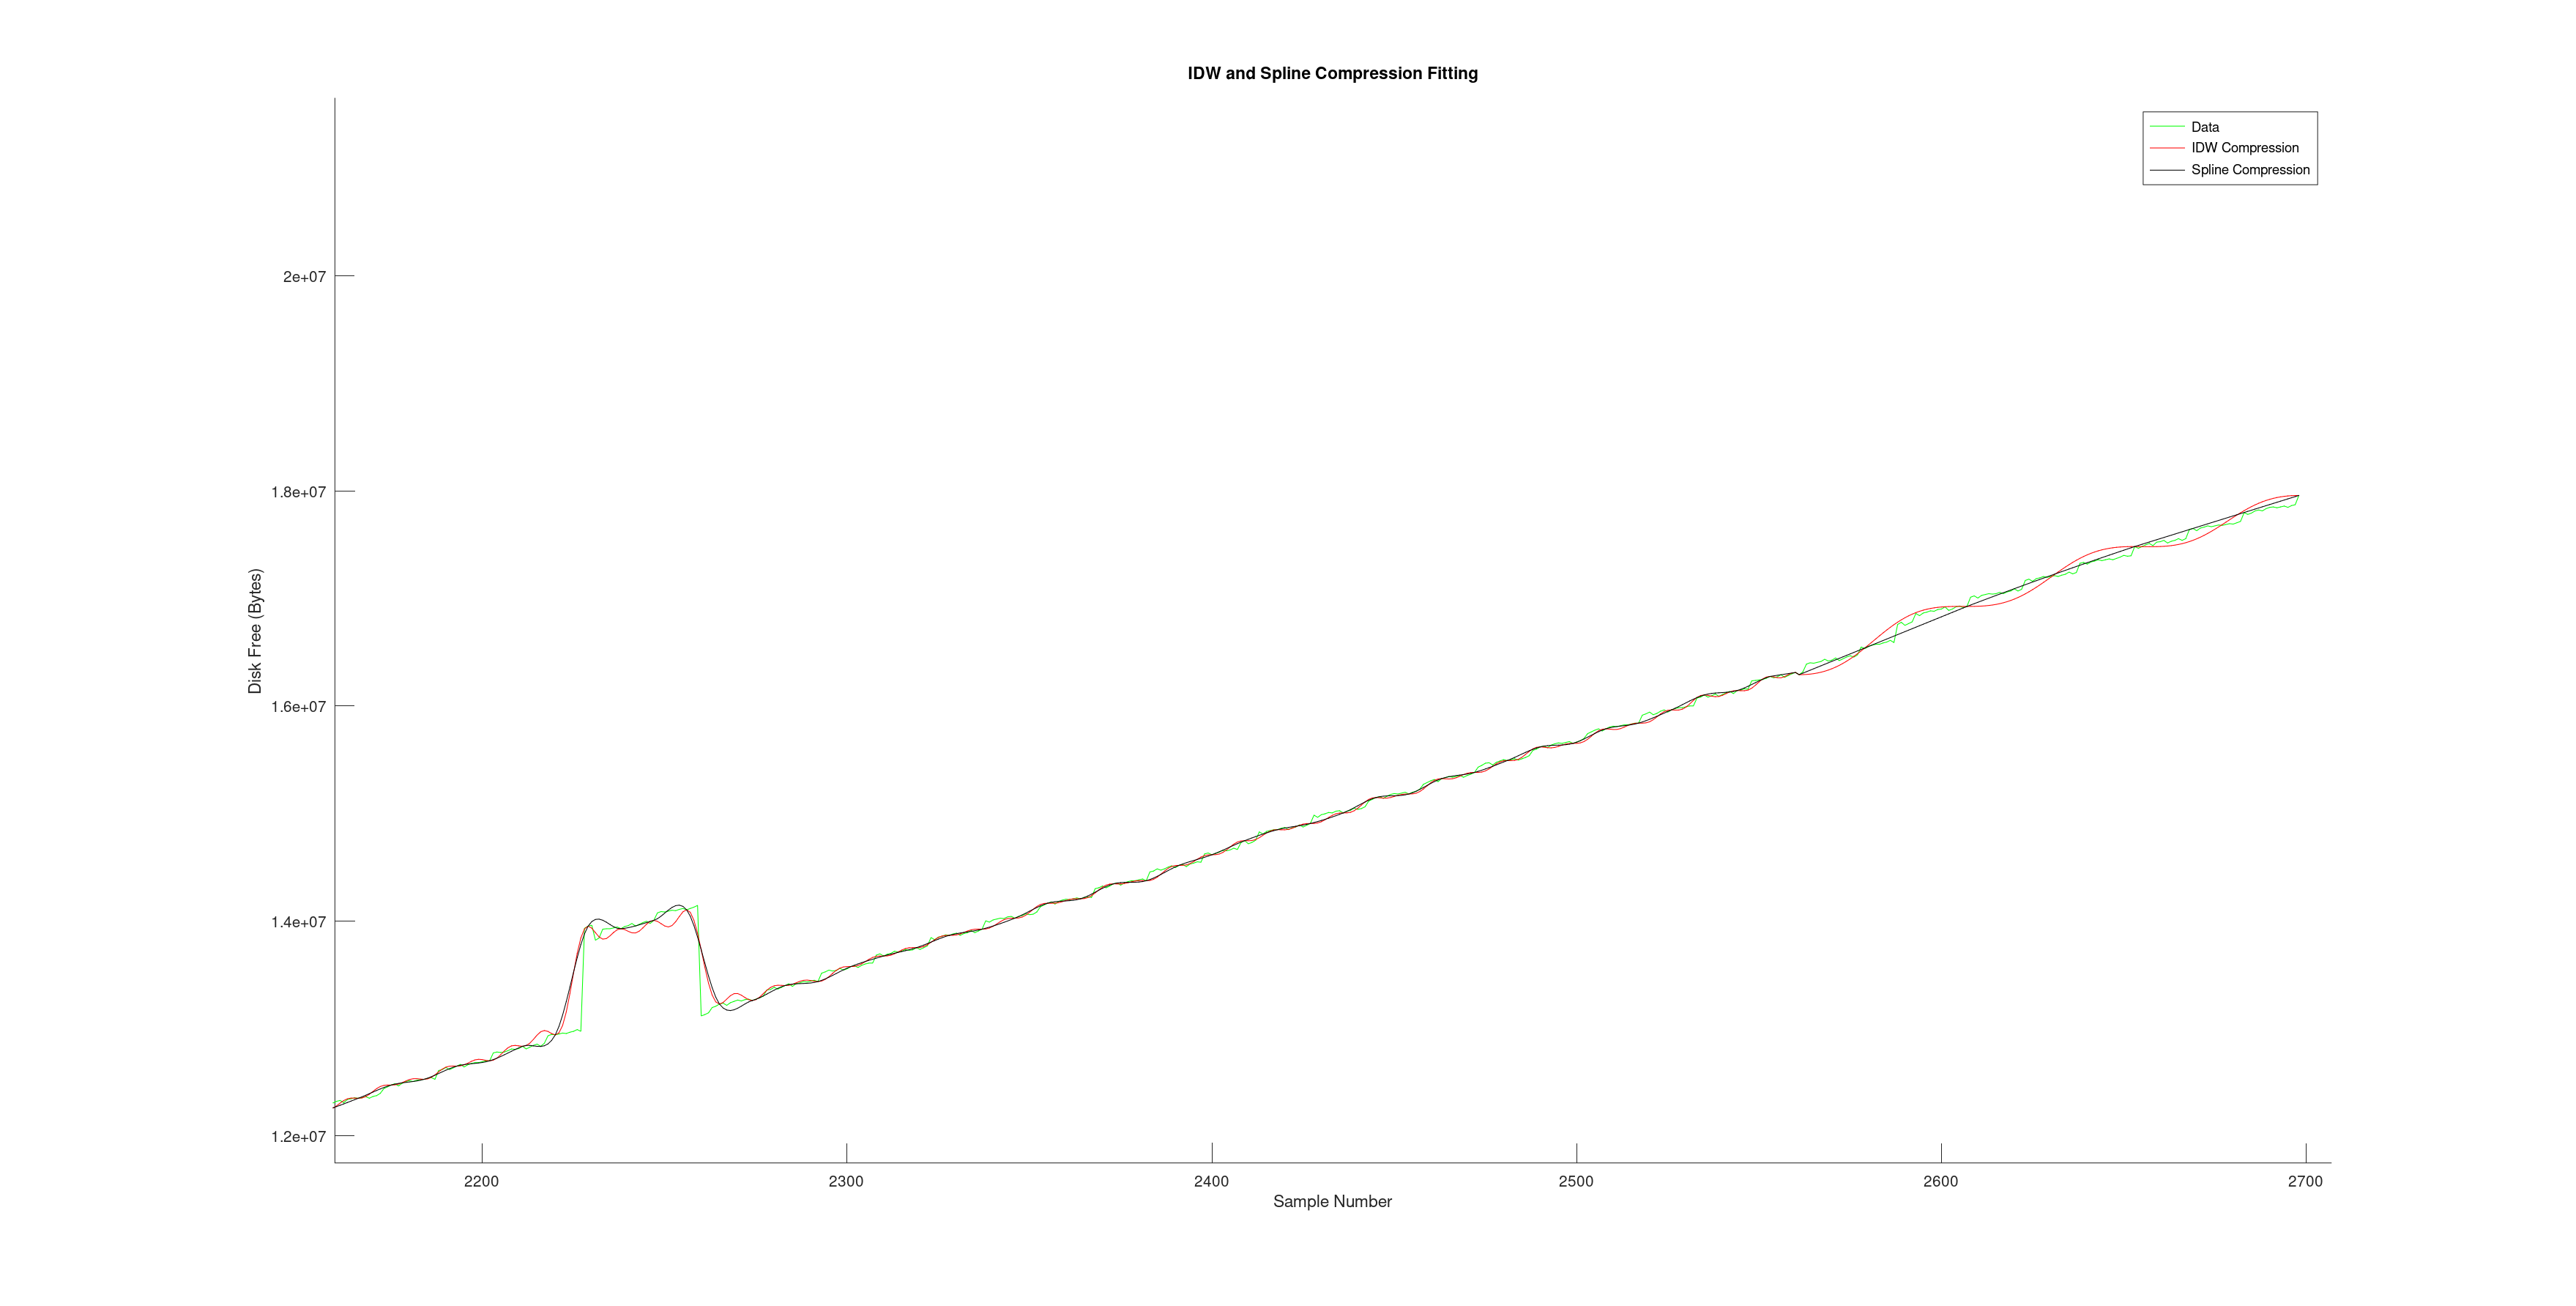
\includegraphics[width=0.5\textwidth]{IDW_Spline_Comparison.png}
  \caption{Signal Fitting of the original data with IDW Compression and Spline Compression (Both 43x compression).}
  \label{Fig.4}
\end{figure}
\vspace{5pt}

\vspace{10pt}
\subsubsection{Linear predictive coding (LPC)}

A lot of lessons were learned from initial experiments with Audio compressors (mostly FLAC encoder).
Good results were obtained and it was a natural approach to include the those within the available compressors.
The approach is exactly the same as described in the FLAC format [11], but with a small change.
The FLAC expects all samples to be integer, as such, floating point signals are discarded and not usable by definition.
But for signals with a very small precision and bounded (e.g. 0.00 - 100.00) we can convert those to integer and use the LPC compressor.
In practical testing, LPC offers worst compression than FFTs, so FFT is widely used, and in a similar case as the Inverse Distance Weighting, it is mostly relegated to a manual selection.
The only case where LPC is used, is in lossless compression, where it offers a very solid compression averaging between 4x to 8x.

\vspace{10pt}
\section{Error Correction}

All the methods described above generate lossy compression. 
For reducing the error of the compression and/or remove artifacts from the generated signals the following process is used:

\begin{itemize}
    \item Error detection via Mean Absolute Percentage
    \item Storing of the errors that are above the defined error threshold
    \item Discard error points until the global error threshold is met. Since the biggest error points are discarded last, the biggest differences are eliminated.
\end{itemize}

For lossless compression all the point differences need to be stored. In a lot of cases this leads to almost no compression unless the signal has a perfect fitting with
the mathematical representation.

\section{Indexing Samples with VRSI (Variable Rate Sampling Interval)}
\vspace{5pt}
\subsubsection{Overview of VRSI Mechanism}

In the methodology section, a critical aspect of the process involves indexing samples for efficient data retrieval. Variable Rate Sampling Interval (VRSI) is employed to manage the sampling intervals effectively. VRSI operates on the premise that samples occur at evenly spaced intervals, such as every 5 seconds, 20 seconds, or 60 seconds.
\vspace{5pt}
\subsubsection{Line Segment Representation}

For each sampling interval, a line segment is created with specific fields:

\begin{itemize}
    \item \textbf{Start Timestamp:} The timestamp marking the beginning of the sampling interval.
    \item \textbf{Sample Interval:} The time gap between consecutive samples.
    \item \textbf{Starting Sample:} The index of the first sample within the segment.
    \item \textbf{Number of Samples:} The total number of samples within the segment.
\end{itemize}
\vspace{5pt}
\subsubsection{File Structure}

These line segments are then stored in a file, accompanied by the lowest and highest timestamps in the segments represented. This file structure allows for easy identification of whether a requested interval is present in the index. If the requested interval falls entirely outside the timestamps in the file header, no samples are available for that interval.
\vspace{5pt}
\subsubsection{Handling Temporal Gaps}

In cases where a metric stops reporting for a period, a new line segment is generated, ensuring accurate representation of the sampled data over time.
\vspace{5pt}
\subsubsection{Example VRSI File Content}

\begin{verbatim}
55745
59435
15,0,55745,166
15,166,58505,63
\end{verbatim}


\begin{itemize}
    \item Line 1) Represents the first timestamp.
    \item Line 2) Represents the last timestamp.
    \item Line segments are detailed below:
    \begin{itemize}
        \item The first line segment has one sample every 15 seconds, starting at timestamp 55745, with a total of 166 samples.
        \item The second line segment also has one sample every 15 seconds, starting at timestamp 58505, with 63 samples.
    \end{itemize}
\end{itemize}
\vspace{5pt}
\subsubsection{Locating Samples (Read Path)}

In the read path, when locating a sample in a file using the index, timestamps or timestamp ranges are specified (e.g., "All the samples from 3:30 PM to 4:30 PM"). The system checks if the requested timestamps are within the available timestamps in the file header. If found, the sequence of sample numbers is extracted, indicating the samples needed for decompression.
\vspace{5pt}
\subsubsection{Creating/Updating the Index (Write Path)}

When a new sample is added, the index is updated. Since time progresses linearly, and samples occur in sequence, the system only needs to:
\begin{itemize}
    \item Update the last segment's sample number or
    \item Create a new segment.
\end{itemize}

Existing segments are incremented if the sample timestamp is the next in sequence. If a segment does not exist or the timestamp is not the next in sequence for the latest segment, a new segment is created. This approach ensures an efficient and organized index for managing variable rate sampling intervals.

\begin{figure}[h]
  \centering
  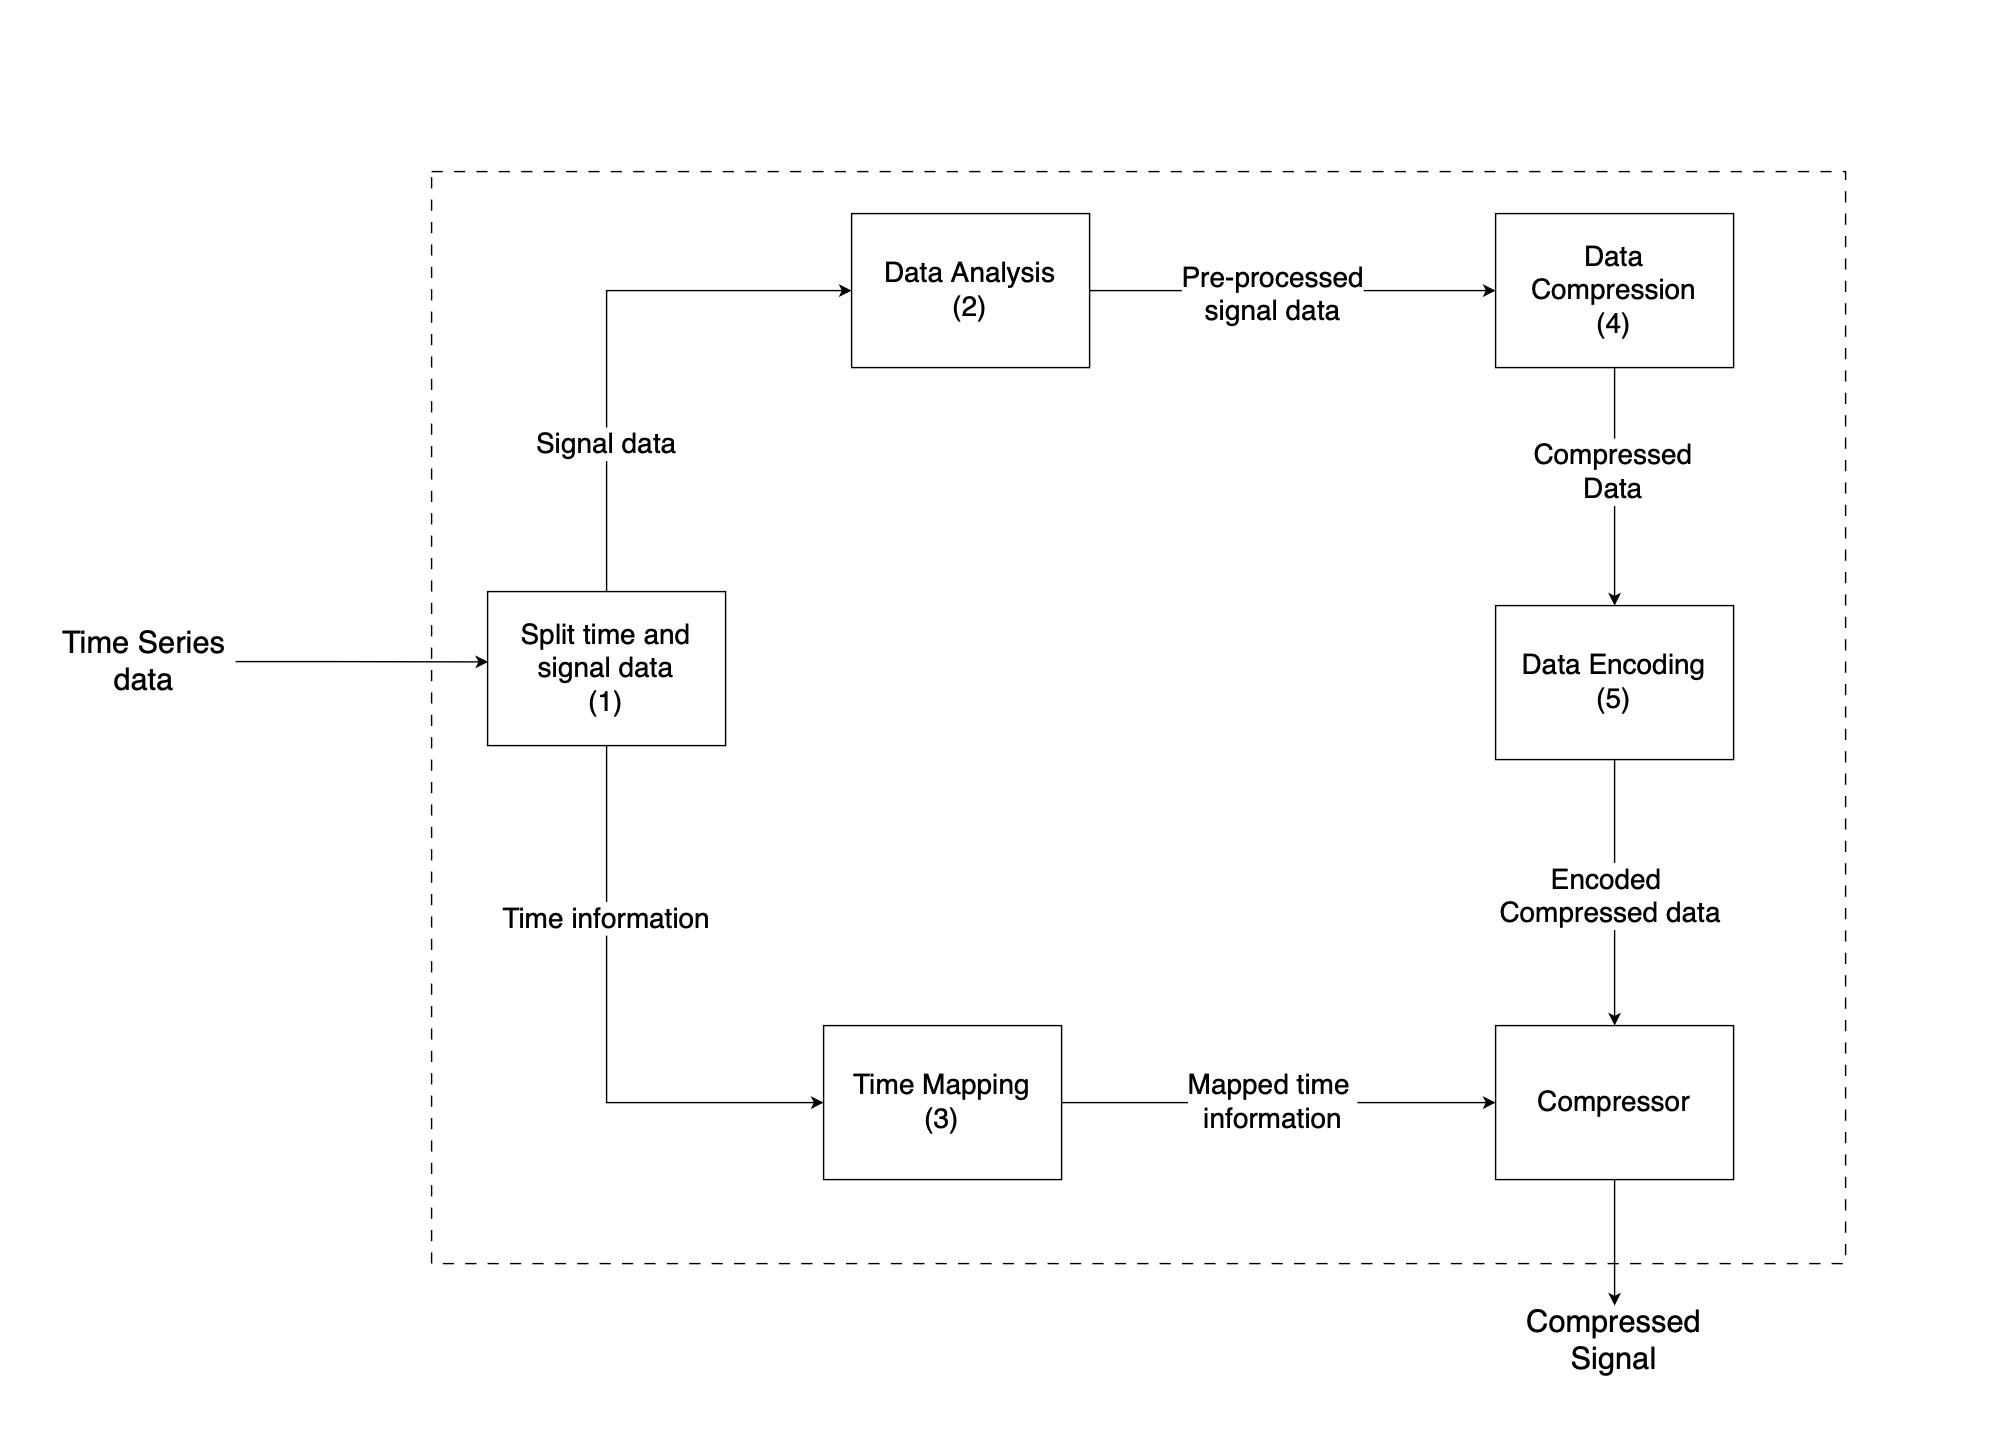
\includegraphics[width=0.5\textwidth]{Fig4.png}
  \caption{Internal Diagram of the ATSC Compressor.}
  \label{Fig.5}
\end{figure}
%% Estou aqui!
\section{Results}

In our quest to assess the efficiency and effectiveness of ATSC, a comprehensive testing methodology was employed. The ATSC server was configured as both a read and write backend for a Prometheus instance, establishing a practical and relevant testing environment. This Prometheus instance, in turn, was connected to an Instaclustr internal production 57-node Cassandra cluster with a Prometheus endpoint enabled. 
The data flow was then collected at the node level, sent to prometheus endpoint that would then forward it to the ATSC server configured as previsously stated.
The server run for approximated 18h over 2 days. Collecting 1 point every 20 sec. This ended with a 5432 samples for each signal, for each node. For a total of 14386 signals processed.
ATSC run with automatic compressor selection and a maximixum allowed error of 3\\%.

\subsection*{ATSC Single: A Best-Case Scenario Analysis}

Before delving into the detailed results, it is essential to address the ATSC single scenario. This represents an optimal output expected on a server running for an extended period, devoid of headers and enriched with substantial data conducive to efficient compression. Although this scenario does not reflect a realistic measure, it serves as a best-case scenario for the current test. The approach involves consolidating all data from every file into a single file, subsequently compressed.

\subsection*{Data Overview}

\textbf{Raw Data Size:} 261,370,032 bytes \\
\textbf{Compression Statistics:}

\begin{itemize}
    \item \textbf{ATSC Compression:}
    \begin{itemize}
        \item Compressed Size: 4,558,363 bytes
        \item Compression Ratio: 57.34 times
    \end{itemize}
    \item \textbf{LZ4 Compression:}
    \begin{itemize}
        \item Compressed Size: 30,634,699 bytes
        \item Compression Ratio: 8.53 times
    \end{itemize}
    \item \textbf{FLAC Compression:}
    \begin{itemize}
        \item Compressed Size: 46,524,174 bytes
        \item Compression Ratio: 5.62 times
    \end{itemize}
\end{itemize}

\textbf{Signal Count:}

\begin{itemize}
    \item Total Signals: 5,860
\end{itemize}

\textbf{Compression Ratios Analysis:}

\begin{itemize}
    \item Median Compression Ratio: 1,653.82
    \item Average Compression Ratio: 1,979.21
\end{itemize}

\begin{figure}[h]
  \centering
  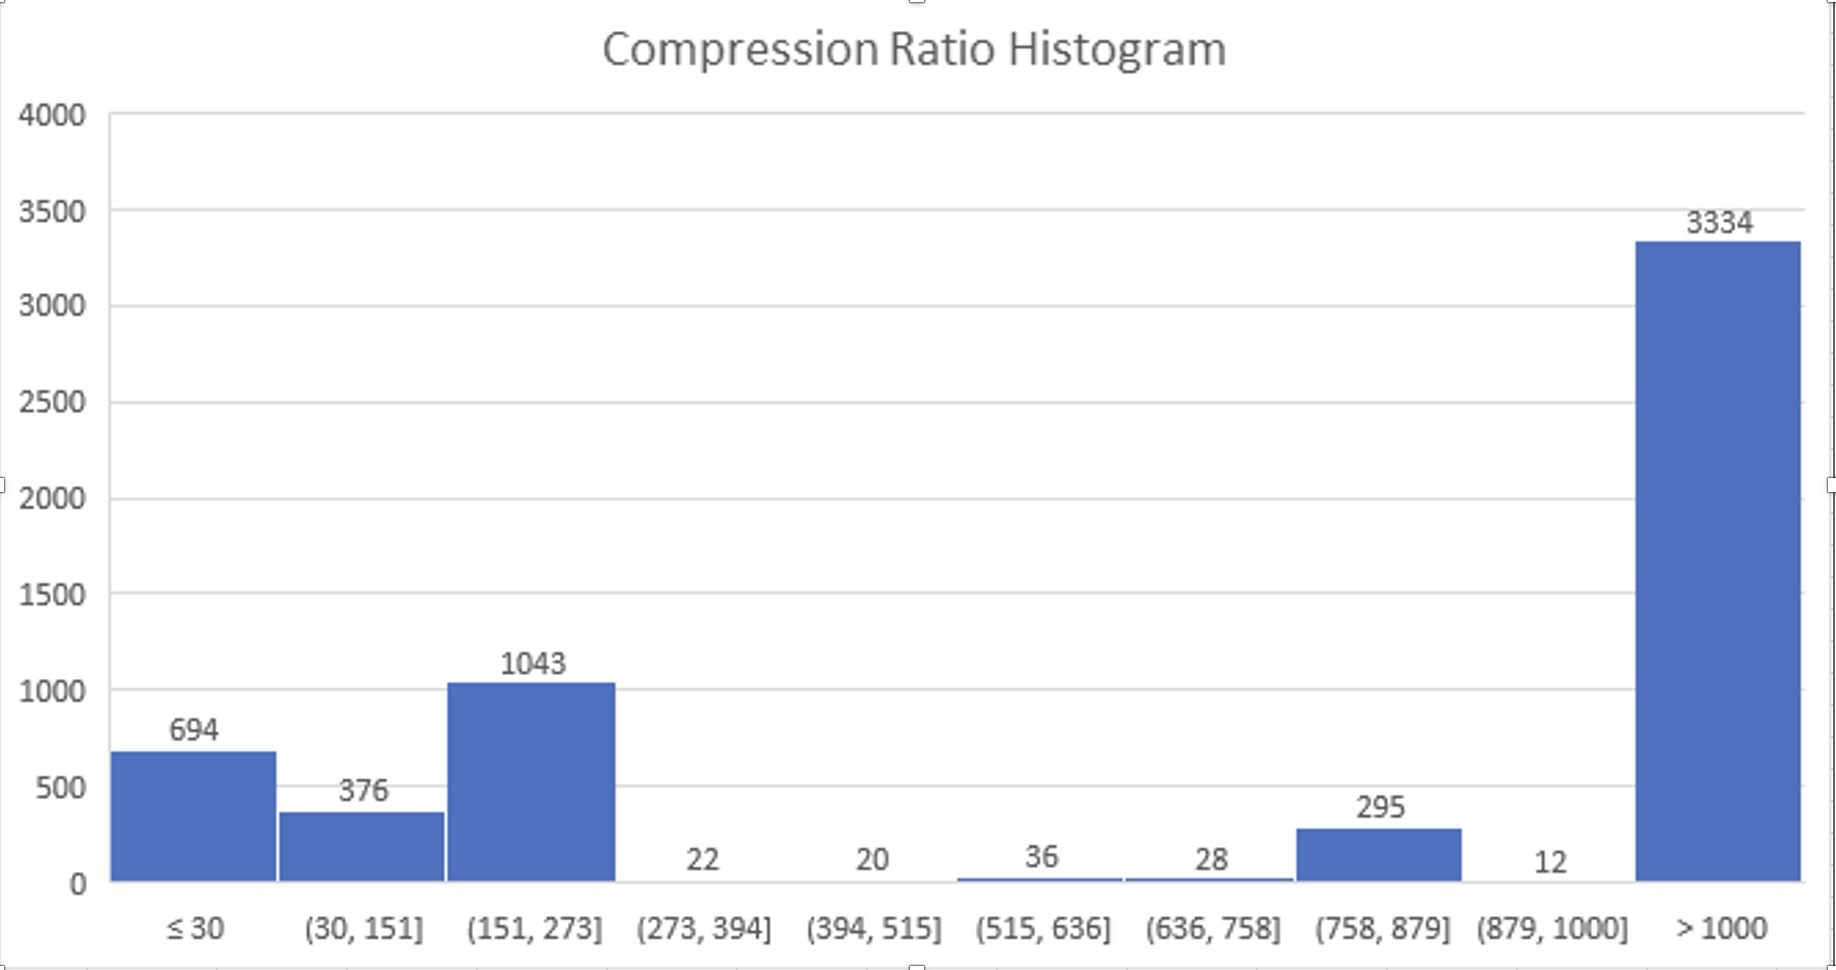
\includegraphics[width=0.5\textwidth]{Fig5.png}
  \caption{Compression Ratio Histogram}
  \label{Fig.6}
\end{figure}

\vspace{10pt}
These results offer a detailed insight into the performance of ATSC across various compression techniques. The data overview provides the baseline, while compression statistics and signal count shed light on the efficiency of ATSC's compression strategies. The analysis of compression ratios, both median and average, further quantifies the compression effectiveness across the tested scenarios. 
 
\subsection{Result validation}

For validation of the results, the data was uncompressed


\begin{figure}[h]
  \centering
  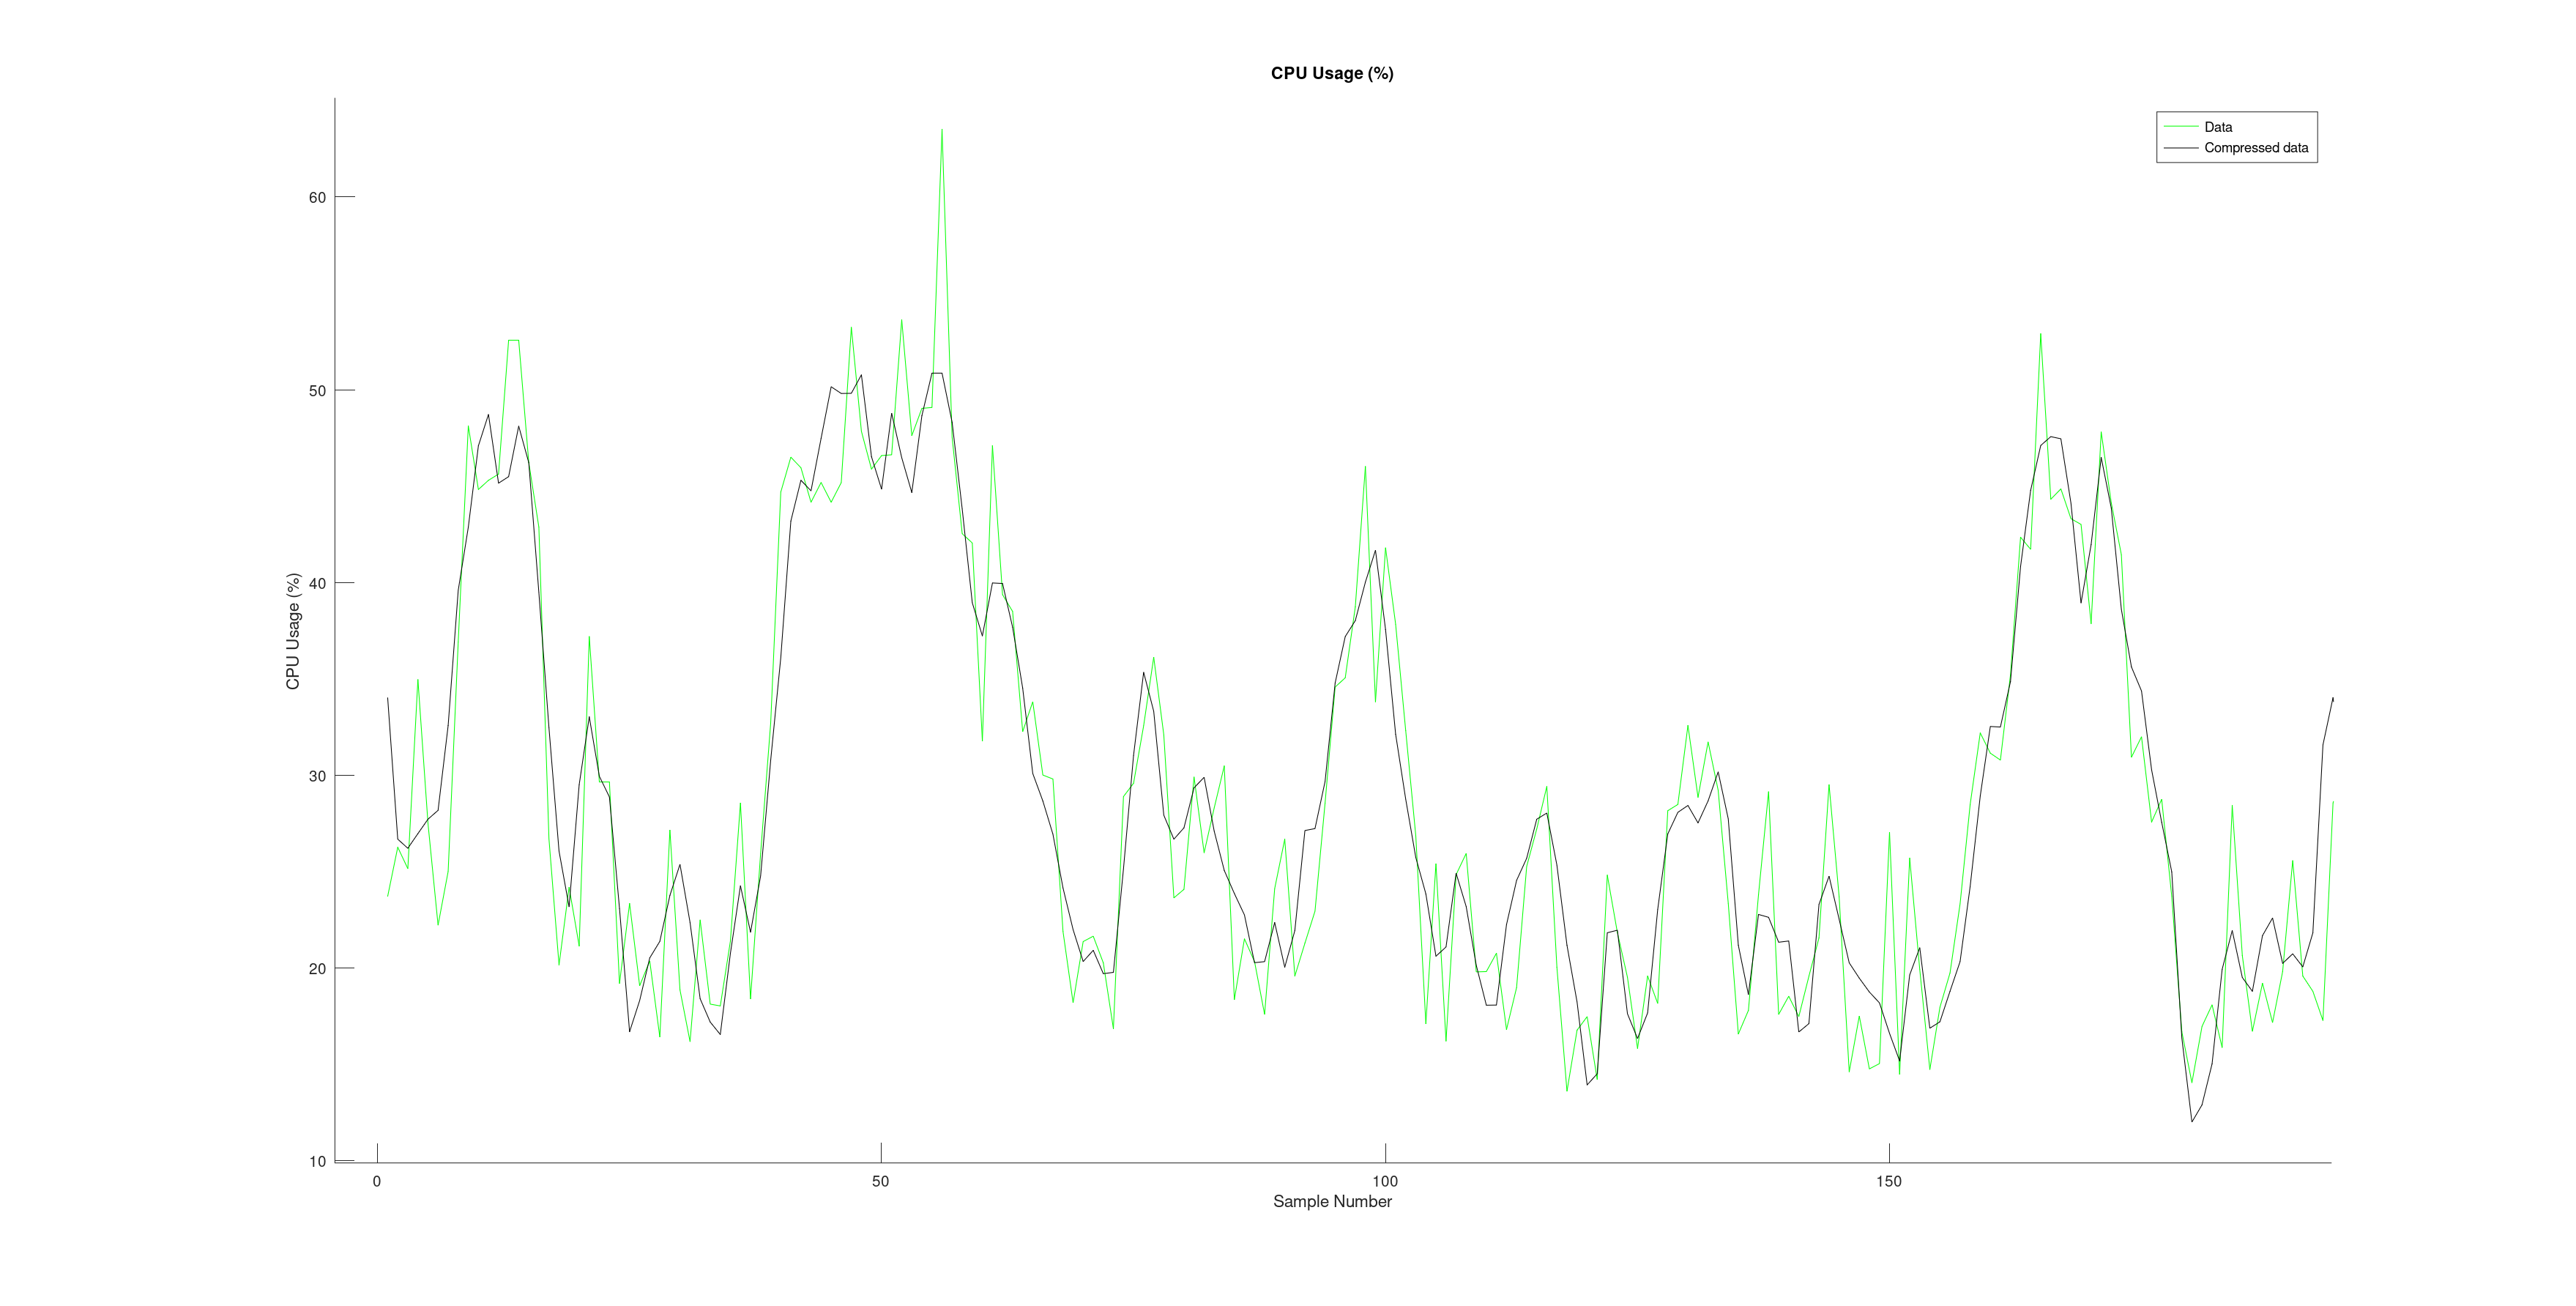
\includegraphics[width=0.5\textwidth]{cpu-usage-validation.png}
  \caption{CPU compression vs Original data}
  \label{cpu}
\end{figure}

\begin{figure}[h]
    \centering
    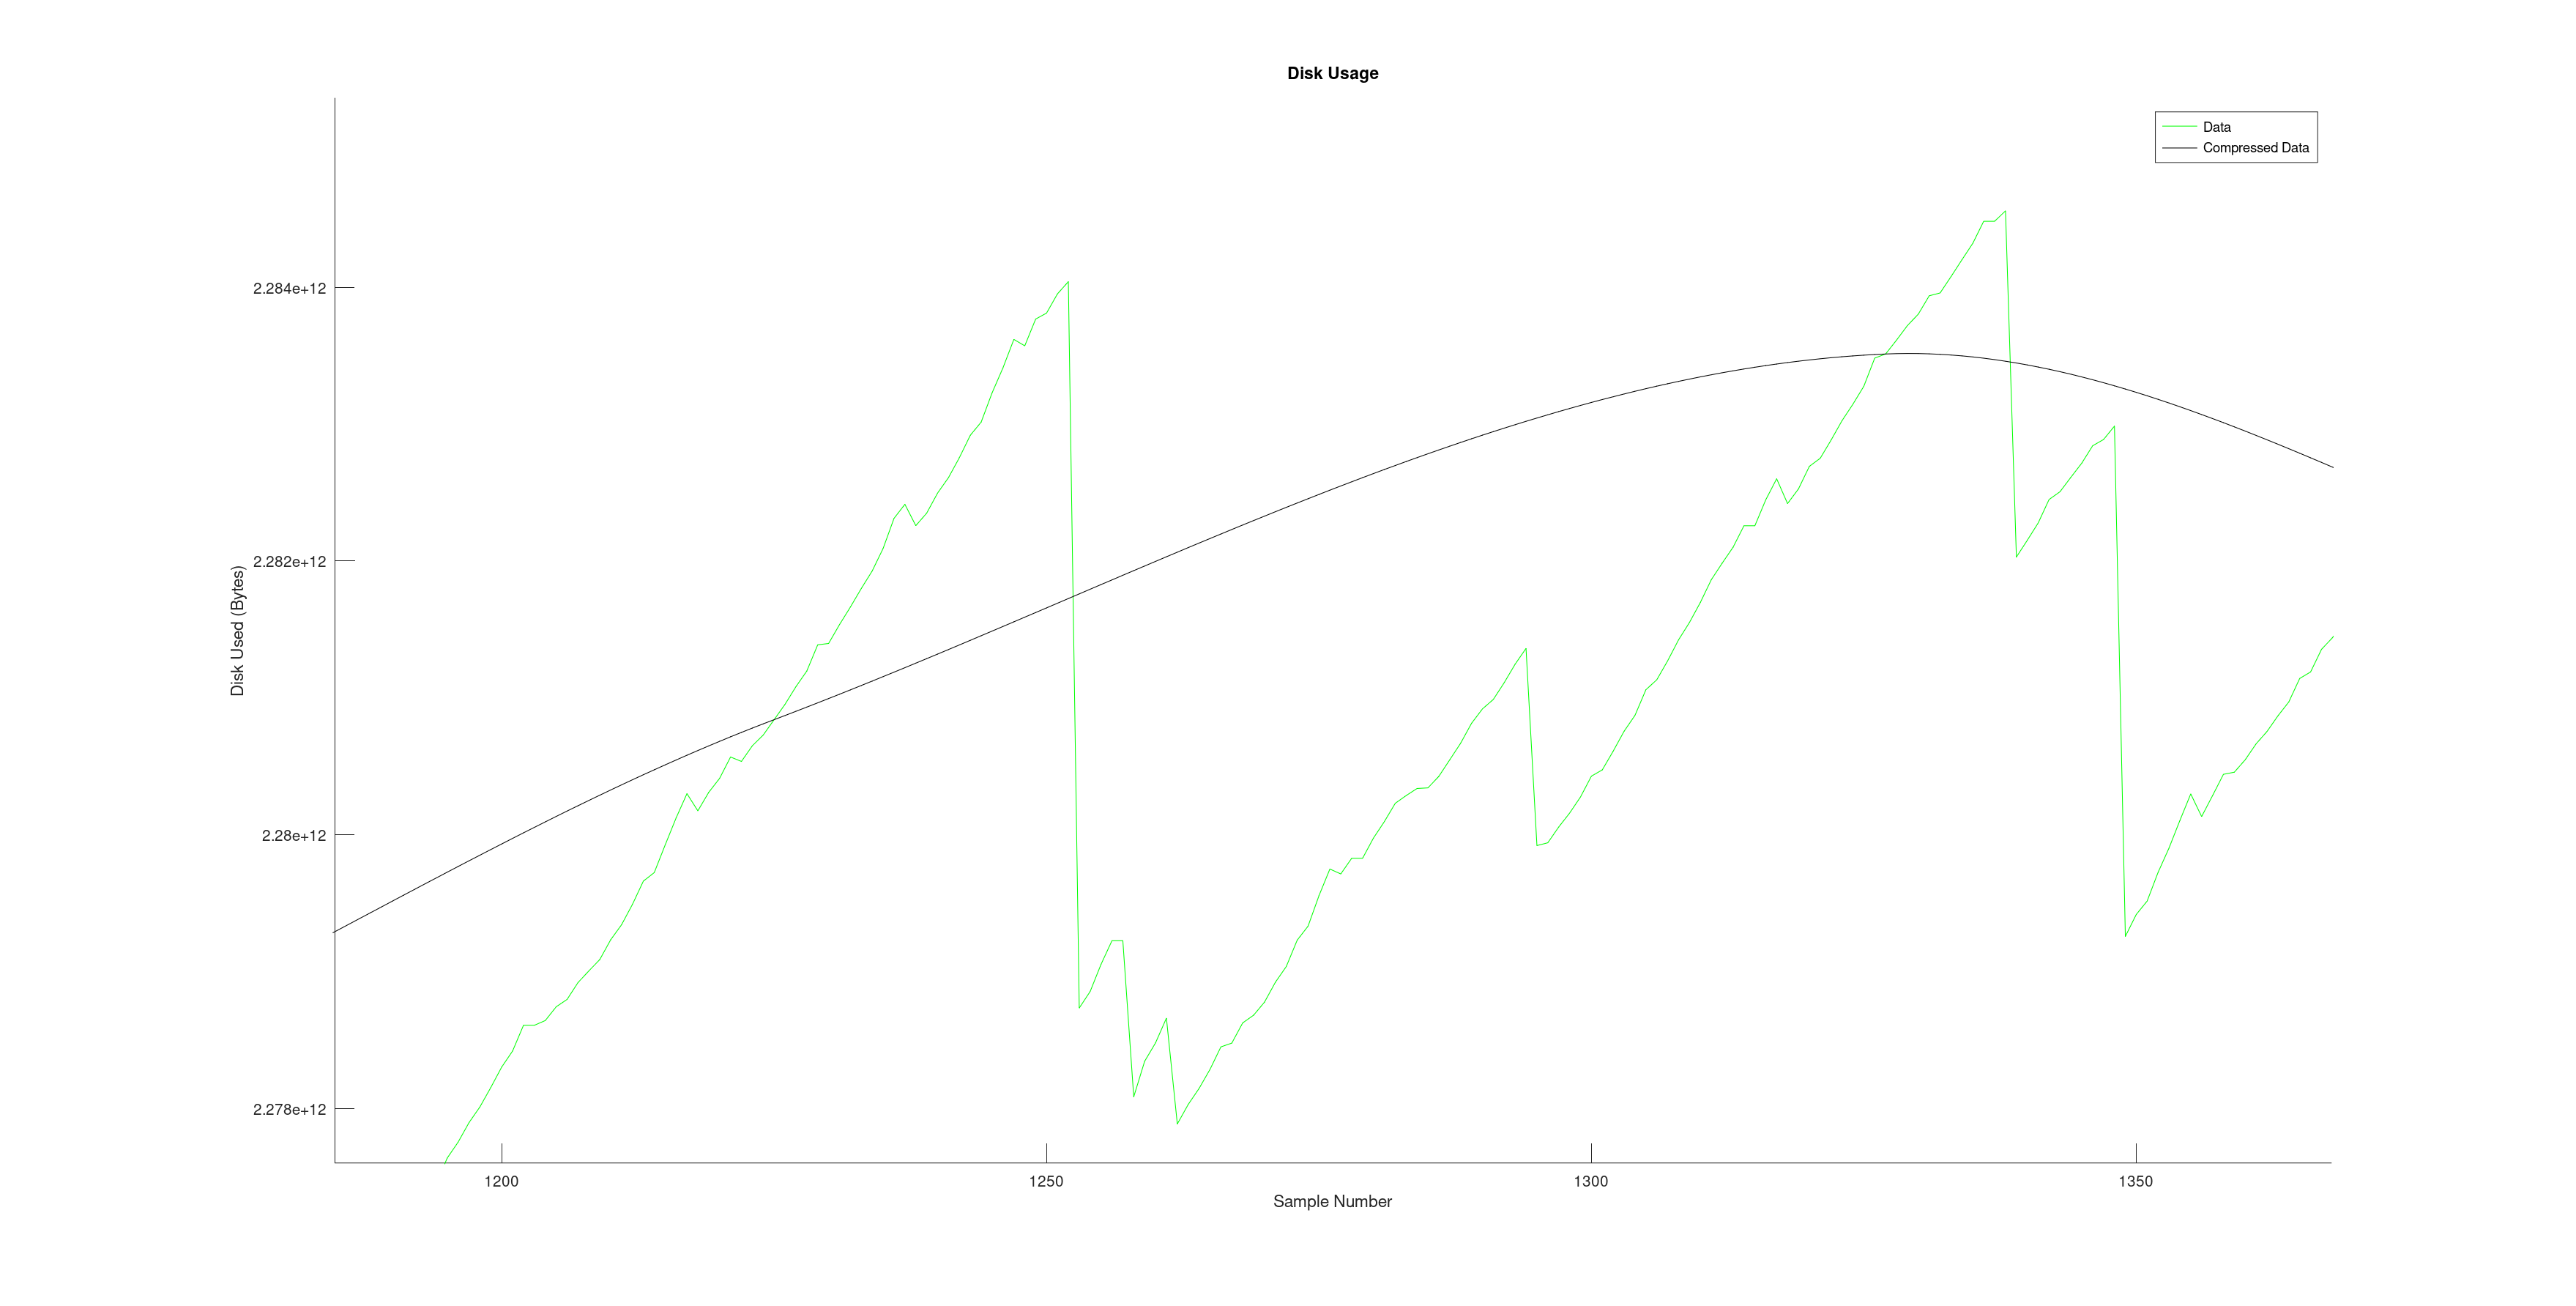
\includegraphics[width=0.5\textwidth]{disk-usage-validation.png}
    \caption{Disk compression vs Original data}
    \label{Disk}
  \end{figure}

  \begin{figure}[h]
    \centering
    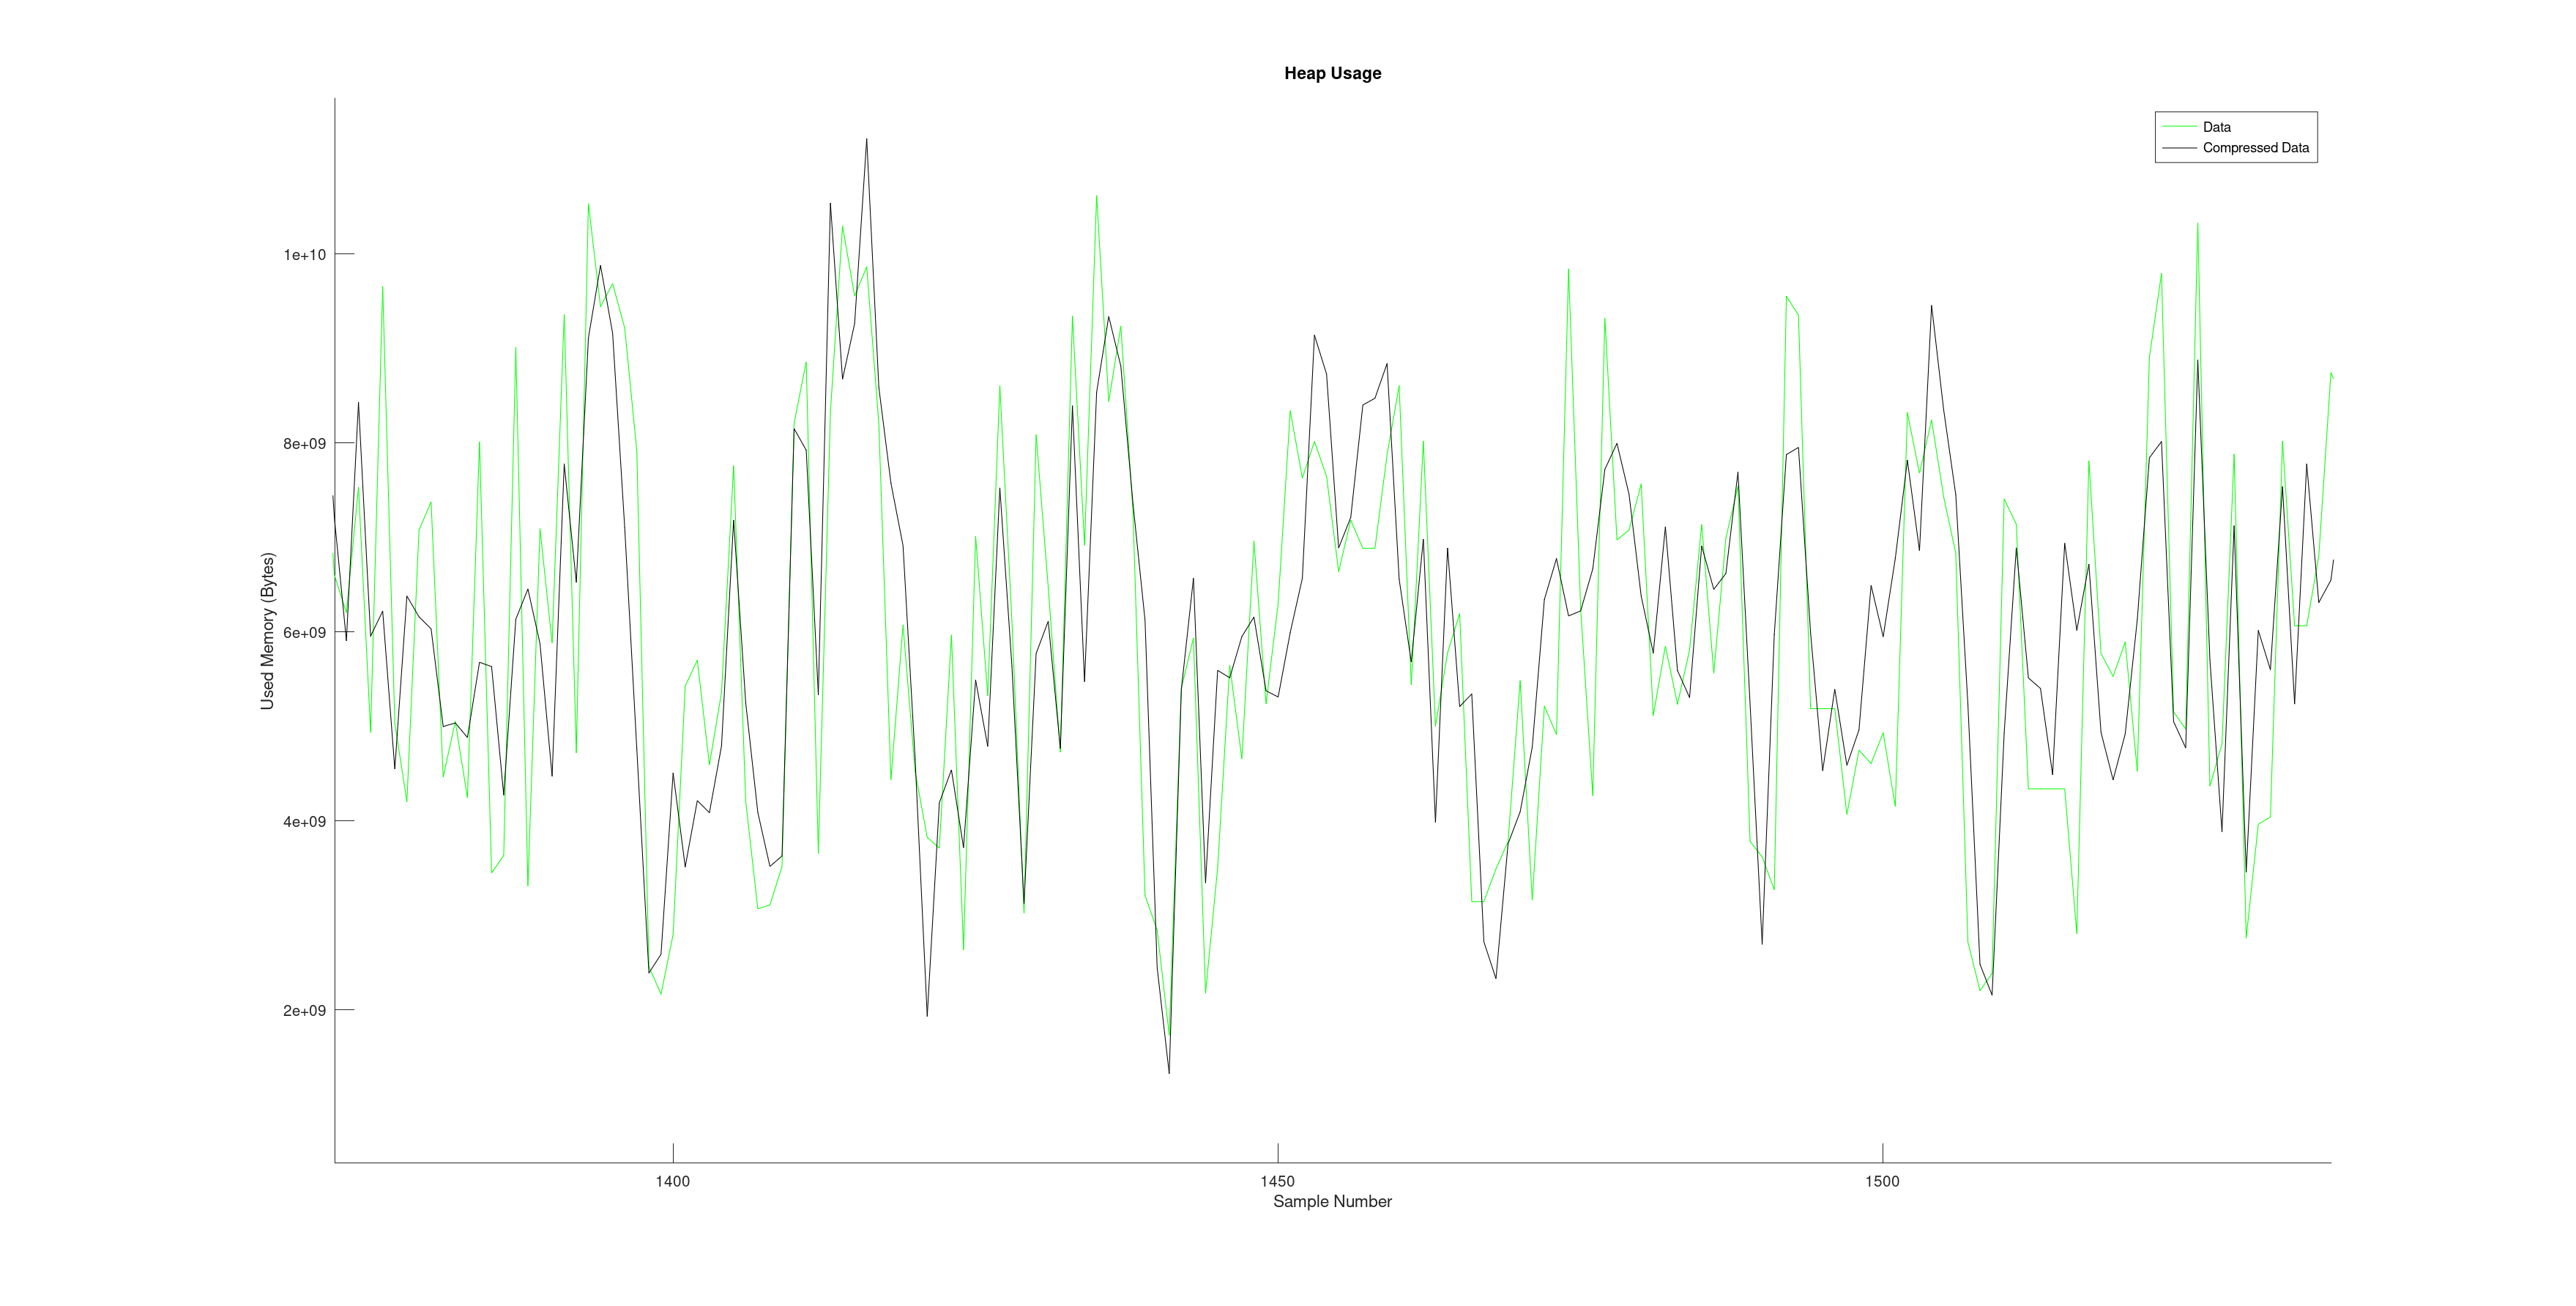
\includegraphics[width=0.5\textwidth]{heap-usage-validation.png}
    \caption{Heap Usage Compressed vs Original data}
    \label{heap}
  \end{figure}
\vspace{10pt}
The ATSC Compression exhibited an impressive compression ratio of 57.34 times, showcasing the potential of BRRO in achieving substantial data reduction. Additionally, the LZ4 and FLAC Compression techniques demonstrated notable compression ratios of 8.53 and 5.62 times, respectively, highlighting the versatility of ATSC in adapting to different compression scenarios. 
These results substantiate ATSC's capabilities in optimizing storage space, offering valuable insights into its potential impact on real-world applications. 

\section{Future Work}

ATSC show a significant improval over existing compression for time-series. But there are several avenues of possible work to further expand its capabilities and/or use some of the opportunities it exposes.

%OLD - In the pursuit of continual improvement and innovation, the following avenues represent promising areas for future exploration within the context of ATSC.

\subsection{AI for compressor selection and optimization}

Currently ATSC has a small subset of fixed algorithms available to chose from. The choice is made based on a simplistic statistical analysis. With a growing number of signals analised it could be possible to use AI to make an optimal choice. 
Also, AI could be used to make a more curated choice of algorithms available for compression.

%OLD - Enhancing User Experience: Investigate the potential benefits of incorporating automated selections, possibly powered by Artificial Intelligence (AI). This exploration aims to streamline user interactions and optimize compression choices intelligently.

\subsection*{Test further algorithms}

ATSC algorithm selection could be expanded alongside improved selection methods, that could further increase ATSC compression ratio.

%OLD - Extend ATSC's functionality by integrating seamlessly with Time Series databases and services. This integration holds the promise of providing users with a cohesive and efficient solution for managing Time Series data.

\subsection{Integration with other systems}

while developing and researching we found that ATSC creates similar outputs for a lot of signals. Compression of a signal signal at a time doesn't allow us to benefit from this. By using ATSC integrated in a database/filesystem/etc it would be possible
to identify such scenarios and avoid storing further once we know a particular output exists already, thus further increase space savings.

%OLD - Building on Experience: Draw insights from early experiments, particularly those involving Free Lossless Audio Codec (FLAC). Utilize the lessons learned to inform and refine ATSC's performance in streaming scenarios.

\subsection{Outlier detection}

One characteristics that was noted during result analysis, as that for systems with a lot of nodes doing the same work (e.g. Cassandra database with multiple nodes), compression ratios for a given metric across all nodes would be mostly the same.
In a couple of cases we found that some nodes had significant differences for some metrics (more than double, sometimes 10x worse compression). By looking into the detailed metrics we could find that the node was misbehaving and it should be fixed 
or replaced. This opens a front worth exploring that is comparing compression ratios for outlier detection.

%OLD - Apply the knowledge gained from FLAC experiments to optimize ATSC's streaming capabilities. This involves fine-tuning the compression strategy to excel in scenarios where real-time or efficient streaming of Time Series data is paramount.
%These future directions underscore ATSC's commitment to continuous improvement and adaptation to emerging technologies. By exploring automated selections, integrating with Time Series databases, and leveraging lessons from streaming experiences, ATSC aims to stay at the forefront of efficient and intelligent Time Series data compression. This forward-looking section sets the stage for ongoing advancements and ensures that ATSC remains a versatile and cutting-edge solution in the dynamic landscape of data compression.


\section{conclusion}

In conclusion, the ATSC approach outlined in this research offers a novel solution for monitoring time series data compression, particularly in computer systems. By using a new approach, ATSC achieves impressive compression ratios, with a best-case scenario reaching over 1000x times compression. This innovative methodology not only addresses current storage and data transfer challenges but also sets the stage for future improvements.
\vspace{5pt}
Preliminary testing against a Production cluster demonstrates significant space savings in the ATSC compared to currently state of the art methods. The research emphasizes the importance of unique indexing for precise data retrieval, showcasing its efficiency in streaming and targeted decompression of relevant data segments.

The outlined future work underscores ATSC's commitment to continuous improvement, with a focus on automated selections, integration with time series databases, and adding other capabilities. These efforts aim to keep ATSC at the forefront of efficient and intelligent time series data compression.

In summary, ATSC emerges as a promising solution that not only tackles current challenges but also paves the way for ongoing advancements in the dynamic landscape of time series data compression.

\section{References}

\begin{enumerate}
    \item InfluxData. (n.d.). What is Time Series Data? [Online]. Available: \url{https://www.influxdata.com/what-is-time-series-data/} [1]

    \item Teller, J., et al. (2015). Gorilla: A Fast, Scalable, In-Memory Time Series Database. Proceedings of the VLDB Endowment, 8(12), 1816-1827. PDF [2]

    \item VictoriaMetrics. (n.d.). Achieving Better Compression for Time Series Data than Gorilla. [Online]. Available: \href{https://faun.pub/victoriametrics-achieving-better-compression-for-time-series-data-than-gorilla-317bc1f95932}{https://faun.pub/victoriametrics-achieving-better-compression-for-time-series-data-than-gorilla-317bc1f95932} [3]

    \item TimeScale. (n.d.). Time Series Compression Algorithms Explained. [Online]. Available: \url{https://www.timescale.com/blog/time-series-compression-algorithms-explained/} [4]

    \item DZone. (n.d.). Time Series Compression Algorithms and Their Applications. [Online]. Available: \url{https://dzone.com/articles/time-series-compression-algorithms-and-their-appli#:~:text=Time%20series%20compression%20algorithms%20take%20advantage%20of%20specific,functions%20or%20predicting%20them%20through%20neural%20network%20models} [5]

    \item Yang, S., et al. (2021). An Intelligent Compression Algorithm for Time Series Data. PDF [6]

    \item Gunasekaran, M., et al. (2019). SmartFusion CSOC Implementation of FLAC Player Using Hardware and Software Partitioning. [Online]. Available: \href{https://www.microsemi.com/document-portal/doc_view/129825-ac376-smartfusion-csoc-implementation-of-flac-player-using-hardware-and-software-partitioning-app-note} [7]

    \item Wikipedia. (n.d.). List of Hardware and Software that Supports FLAC. [Online]. Available: \url{https://en.wikipedia.org/wiki/List_of_hardware_and_software_that_supports_FLAC} [8]

    \item Apache Cassandra. (n.d.). Operating Metrics. [Online]. Available: \url{https://cassandra.apache.org/doc/latest/cassandra/operating/metrics.html} [9]

    \item Free Patents Online. (n.d.). Data Compression Method and Apparatus. [Online]. Available: \url{https://www.freepatentsonline.com/5839100.html} [10]

    \item Free Lossless Audio Codec \url{https://datatracker.ietf.org/doc/html/draft-ietf-cellar-flac-14#name-prediction} [11]
\end{enumerate}

\end{document}